 % The main file for CAMP reports
 % Don't put any content in here. 
 % Don't even include content files by using \input or \inlcude. 
 % Put your content to TEXT.TEX or include it there using \input.
 % Uses:
 %		SETTINGS.TEX	contains the settings for this document
 %		COMMANDS.TEX	contains commands which can be used while writing
 %		INFO.TEX			contains the author, title and so on for the cover
 %		COVER.TEX			formats the front cover of the document
 %		ABSTRACT.TEX	contains the abstract to be included (if needed)
 %		TEXT.TEX			contains the actual content of the document
 %		BIB.BIB				containt the BibTeX entries for the document
 
 
%% Draft document mode
%% Final document
\documentclass[11pt,headsepline,footsepline,footinclude=false,DIV13]{scrreprt}

% KOMA-Optionen:
%  bibtotoc: include bibliography in table of contents
%  idxtotoc: include index in table of contents
%  headsepline: use horizontalline under heading
%  BCOR: binding correcion (Bindungskorrektur) (e.g.: BCOR5mm)
%  DIV: Number of sheet sections (used for layout) (e.g.: DIV12) 



% include title and author information for the cover
% Set here the title, authors and other stuff to be used for the cover
% This file is used by MAIN.TEX

% set title, authors and stuff for the cover
\def\doctype{IDP - Physics}
\def\title{Development and implementation of the data and slow control acquisition system for the TUM neutron electric dipole moment (nEDM) experiment}
%\def\titleGer{ }
\def\author{Thomas Reschenhofer \\[2mm] Bernhard Waltl}
\def\date{April 15, 2013}

% text to appear in the footer
\def\footertext{}

% include settings
% Included by MAIN.TEX
% Defines the settings for the CAMP report document

\renewcommand{\sectfont}{\normalfont \bfseries}        % Schriftart der Kopfzeile

% manipulate footer
\usepackage[headsepline,plainheadsepline,automark]{scrpage2}
%\usepackage{scrpage2}
\pagestyle{scrheadings}
\ohead[\pagemark]{\pagemark} \ihead[]{\headmark} \chead{} \cfoot[]{}
\ifoot[\footertext]{\footertext} % \footertext set in INFO.TEX
%\setkomafont{pagehead}{\normalfont\rmfamily}
\setkomafont{pagenumber}{\normalfont\rmfamily}




%% allow sophisticated control structures
\usepackage{ifthen}

% use Palatino as default font
\usepackage{palatino}

% enable special PostScript fonts
\usepackage{pifont}

% make thumbnails
\usepackage{thumbpdf}

%to use the subfigures
\usepackage{subfigure}


\usepackage{styles/colortbl}

\usepackage{listings}


%% show program code\ldots
%\usepackage{verbatim}
%\usepackage{program}

%% enable TUM symbols on title page
\usepackage{styles/tumlogo}


\usepackage{multirow}

%% use colors
\usepackage{color}

%% make fancy math
\usepackage{amsmath}
\usepackage{amsfonts}
\usepackage{amssymb}
\usepackage{textcomp}
\usepackage{styles/yhmath} % f�r die adots 
%% mark text as preliminary
%\usepackage[draft,german,scrtime]{prelim2e}

%% create an index
\usepackage{makeidx}

% for the program environment
\usepackage{float}

%% load german babel package for german abstract
%\usepackage[german,american]{babel}
\usepackage[german,english]{babel}
\selectlanguage{english}

% use german characters as well
\usepackage[latin1]{inputenc}       % allow Latin1 characters

% use initals dropped caps - doesn't work with PDF
%\usepackage{styles/dropping}


%\usepackage{styles/shortoverview}
%----------------------------------------------------
%      Graphics and Hyperlinks
%----------------------------------------------------

%% check for pdfTeX
\ifx\pdftexversion\undefined
 %% use PostScript graphics
 \usepackage[dvips]{graphicx}
 \DeclareGraphicsExtensions{.eps,.epsi}
 \graphicspath{{figures/}{figures/review}} 
 %% allow rotations
 \usepackage{rotating}
 %% mark pages as draft copies
 %\usepackage[english,all,light]{draftcopy}
 %% use hypertex version of hyperref
 \usepackage[hypertex,hyperindex=false,colorlinks=false]{hyperref}
\else %% reduce output size \pdfcompresslevel=9
 %% declare pdfinfo
 %\pdfinfo { 
 %  /Title (my title) 
 %  /Creator (pdfLaTeX) 
 %  /Author (my name) 
 %  /Subject (my subject	) 
 %  /Keywords (my keywords)
 %}
 %% use pdf or jpg graphics
 \usepackage[pdftex]{graphicx}
 \DeclareGraphicsExtensions{.jpg,.JPG,.png,.pdf,.eps}
 \graphicspath{{figures/}} 
 
 %% Load float package, for enabling floating extensions
 \usepackage{float}
 \usepackage{listings}
 %% allow rotations
 \usepackage{rotating}
 %% use pdftex version of hyperref
 \usepackage[pdftex,colorlinks=false,linkcolor=red,citecolor=red,%
 anchorcolor=red,urlcolor=red,bookmarks=true,%
 bookmarksopen=true,bookmarksopenlevel=0,plainpages=false%
 bookmarksnumbered=true,hyperindex=false,pdfstartview=%
 ]{hyperref}
%
%\usepackage[pdftex,colorlinks=false,linkcolor=red,citecolor=red,%
% anchorcolor=red,urlcolor=red,bookmarks=true,%
% bookmarksopen=true,bookmarksopenlevel=0,plainpages=false%
% bookmarksnumbered=true,hyperindex=false,pdfstartview=%
% ]{hyperref}
\fi




%% Fancy chapters
%\usepackage[Lenny]{fncychap}
%\usepackage[Glenn]{fncychap}
%\usepackage[Bjarne]{fncychap}

%\usepackage[avantgarde]{quotchap}

% set the bibliography style
%\bibliographystyle{styles/bauermaNum}
%\bibliographystyle{alpha}
\bibliographystyle{plain}

\setcounter{secnumdepth}{4}
\setcounter{tocdepth}{4}

\lstdefinelanguage{shell}
{
  showspaces=false,               % show spaces adding particular underscores
  showstringspaces=false,         % underline spaces within strings
  showtabs=false,                 % show tabs within strings adding particular underscores
  %keywordstyle=\color{blue},
  morekeywords={},
  otherkeywords={-o, -src, -db, -tbl, -csv, -code, -dest}
  }
	
\lstdefinelanguage{json}
{ showspaces=false,               % show spaces adding particular underscores
  showstringspaces=false,         % underline spaces within strings
	showtabs=false,   
	sensitive=true,
	stringstyle=\color{red},
	keywordstyle=\color{blue},
	morekeywords={true,false,null},
	morestring=[b]"}
	
\lstset{language=C++,
                basicstyle=\ttfamily,
                keywordstyle=\color{blue}\ttfamily,
                stringstyle=\color{red}\ttfamily,
                commentstyle=\color{green}\ttfamily,
                morecomment=[l][\color{magenta}]{\#}
}

% include commands
% Commands to be used within the TUM report document
% Included by MAIN.TEX
% Please include your own cool commands here. 
% Be only sure to comment it sufficiently so others can use it.

%-------------------------------------------------------------
%                      Own Commands
%-------------------------------------------------------------


%-------------------------------------------------------------
% math stuff -------------------------------------------------

% nice R, N, C
\newcommand{\nat}{\mathbb{N}}
\newcommand{\real}{\mathbb{R}}
\newcommand{\compl}{\mathbb{C}}



% norm
\newcommand{\norm}[1]{\left\| #1 \right\|}

% un demi
\newcommand{\half}{\frac{1}{2}}

% parantheses
\newcommand{\parenth}[1]{ \left( #1 \right) }
\newcommand{\bracket}[1]{ \left[ #1 \right] }
\newcommand{\accolade}[1]{ \left\{ #1 \right\} }
%\newcommand{\angle}[1]{ \left\langle  #1 \right\rangle }

% partial derivative: %#1 function, #2 which variable
% simple / single line version
\newcommand{\pardevS}[2]{ \delta_{#1} f(#2) }
% fraction version
\newcommand{\pardevF}[2]{ \frac{\partial #1}{\partial #2} }

% render vectors: 3 and 4 dimensional
\newcommand{\veciii}[3]{\left[ \begin{array}[h]{c} #1 \\ #2 \\ #3	\end{array} \right]}
\newcommand{\veciv}[4]{\left[ \begin{array}[h]{c} #1 \\ #2 \\ #3 \\ #4	\end{array} \right]}

% render matrices: 3  dimensional (arguments in row first order)
\newcommand{\matiii}[9]{\left[ \begin{array}[h]{ccc} #1 & #2 & #3 \\ #4 & #5 & #6 \\ #7 & #8 & #9	\end{array} \right]}
%DOESN'T WORK,DON'T KNOW WHY \newcommand{\mativ}[16]{\left[ \begin{array}[h]{cccc} #1 & #2 & #3 & #4 \\ #5 & #6 & #7 & #8 \\ #9 & #10 & #11 & #12 \\ #13 & #14 & #15 & #16 \end{array} \right]}


%-------------------------------------------------------------
%-------------------------------------------------------------


%-------------------------------------------------------------
% some abreviations ------------------------------------------
\newcommand{\Reg}{$^{\textregistered}$}
\newcommand{\reg}{$^{\textregistered}$ }
\newcommand{\Tm}{\texttrademark}
\newcommand{\tm}{\texttrademark~}
\newcommand {\bsl} {$\backslash$}

%-------------------------------------------------------------
%-------------------------------------------------------------


%-------------------------------------------------------------
% formating --------------------------------------------------

% Theorem & Co environments and counters
\newtheorem{theorem}{Theorem}[chapter]
\newtheorem{lemma}[theorem]{Lemma}
\newtheorem{corollary}[theorem]{Corollary}
\newtheorem{remark}[theorem]{Remark}
\newtheorem{definition}[theorem]{Definition}
\newtheorem{equat}[theorem]{Equation}
\newtheorem{example}[theorem]{Example}
\newtheorem{algorithm}[theorem]{Algorithm}

% inserting figures
\newcommand{\insertfigure}[4]{ % Filename, Caption, Label, Width percent of textwidth
	\begin{figure}[htbp]
		\begin{center}
			\includegraphics[width=#4\textwidth]{#1}
		\end{center}
		\vspace{-0.4cm}
		\caption{#2}
		\label{#3}
	\end{figure}
}




% referecing figures

\newcommand{\refFigure}[1]{ %label
	figure \ref{#1}
}
\newcommand{\refChapter}[1]{ %label
	chapter \ref{#1}
}

\newcommand{\refSection}[1]{ %label
	section \ref{#1}
}

\newcommand{\refParagraph}[1]{ %label
	paragraph \ref{#1}
}

\newcommand{\refEquation}[1]{ %label
	equation \ref{#1}
}

\newcommand{\refTable}[1]{ %label
	table \ref{#1}
}




\newcommand{\rigidTransform}[2]
{
	${}^{#2}\!\mathbf{H}_{#1}$
}

%code, in typewriter
\newcommand{\code}[1]
 {\texttt{#1}}

% comment that appears on the border - very practical !!!
\newcommand{\comment}[1]{\marginpar{\raggedright \noindent \footnotesize {\sl #1} }}

% page clearing
\newcommand{\clearemptydoublepage}{%
  \ifthenelse{\boolean{@twoside}}{\newpage{\pagestyle{empty}\cleardoublepage}}%
  {\clearpage}}


%-------------------------------------------------------------
%-------------------------------------------------------------


\newcommand{\etAl}{\emph{et al.}\mbox{ }}

\newcommand{\shellcmd}[1]{\indent\indent\texttt{\footnotesize\# #1}}


\begin{document}

	% The titlepage for the CAMP report document.
% Included by MAIN.TEX


%--------------------------------------------------
% The title page
%--------------------------------------------------

% correct BCOR - undo at the end !!!
\def\bcorcor{0.15cm}
\addtolength{\hoffset}{\bcorcor}

\thispagestyle{empty}

 \vspace{10mm}
\begin{center}
	       \oTUM{4cm}
	   
	   \vspace{5mm}     
	%   \huge FAKULT{\"A}T F{\"U}R INFORMATIK\\ 
	   \huge INSTITUT F{\"U}R INFORMATIK \\
	   \vspace{0.5cm}
	 \large DER TECHNISCHEN UNIVERSIT{\"A}T M{\"U}NCHEN\\
        
	\end{center}
		

\vspace{10mm}
\begin{center}

   {\Large \doctype}

  \vspace{10mm}
  
  {\LARGE \title}\\
  
  
  \vspace{10mm}
  
  
%  {\LARGE  \titleGer}\\
  
  
  \vspace{10mm}

    %\hfill
    \begin{tabular}{ll}
	   \Large Authors:     & \Large Thomas Reschenhofer \\[2mm]
	   \Large             & \Large Bernhard Waltl \\[2mm]
	   \Large Supervisor:    & \Large Prof. Dr. Peter Fierlinger \\[2mm]				
	   \Large Advisor:	& \Large Dr. Michael Marino\\[2mm]
	   \Large Date:       & \Large April 15, 2013
	 \end{tabular}
	 
	 \vspace{15mm}
	 
	 \begin{figure}[h!]
  \centering
	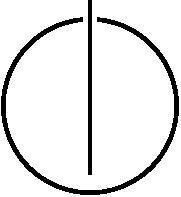
\includegraphics[width=3cm]{images/Informatik.png}
	\hspace{1cm}
	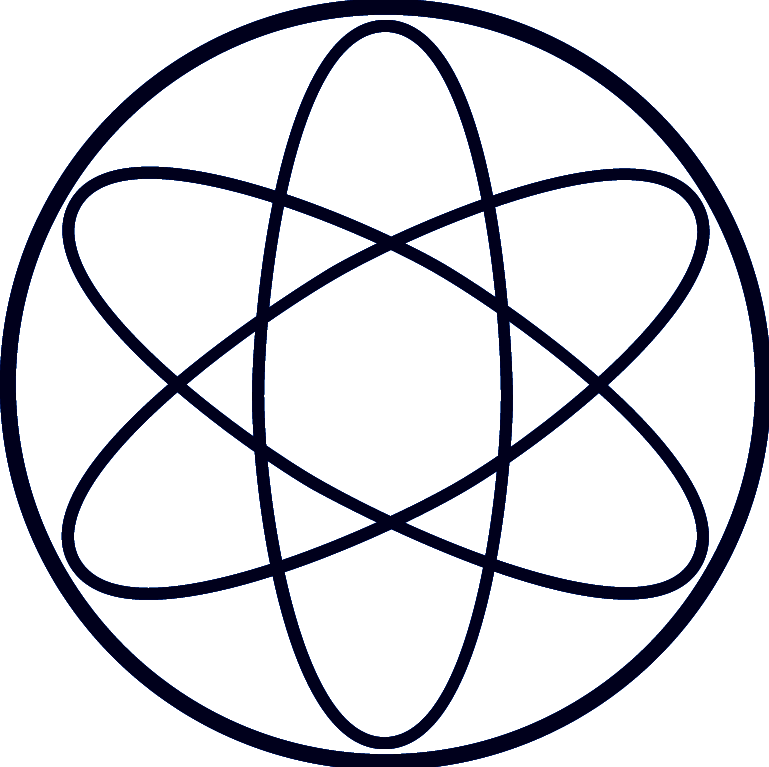
\includegraphics[width=3cm]{images/Physik2.png}
  \end{figure}
   

\end{center}

% undo BCOR correction
\addtolength{\hoffset}{\bcorcor}
	\tableofcontents
  
		% ---------------------------------------------------------------------------
		%
		%Introduction and Background Theory
		%
		% ---------------------------------------------------------------------------
		
		\chapter*{Abstract}

The universe consists of matter (protons, neutrons, etc.) as well as antimatter (antiprotons, antineutrons, etc.). If a particle collides with its respective antiparticle, these matter--antimatter particles are transformed into new force--carrier particles (e.g. photons, gluons, etc.). Therefore, if we assume, that the big bang created both, matter and antimatter equally, all matter and antimatter in the universe would have be transformed to force--carrier particles, whereby we should not exist. However, our existence implies that the amount of matter has to be higher than the amount of antimatter--we would not exist otherwise. This matter--antimatter asymmetry is one of the biggest unsolved problems in physics.\\

To solve this problem, Andrei Sakharov proposed in 1967 a set of three necessary conditions, which lead, if satisfied simultaneously, to an explanation of this asymmetry at an early stage of the universe. The third of them is the violation of the charge symmetry (C) and the charge-parity symmetry (CP), whereas C violation is already known. The CP violation could be verified by the non-zero neutron electric dipole moment (nEDM) experiment, taking place at the Garching Research Centre.\\

In the nEDM experiment, so--called ultra--cold neutrons (UCN) are used, which can be stored in traps made from certain materials because of their small kinetic energy. After their generation, the UCNs are guided into the nEDM measurement chamber. The measurement uses Ramsey's method of separated oscillatory fields applied to UCN in a double--chamber layout, combined with different means of magnetometry. So, if the experiment shows a non-zero value of the neutron's electric dipole moment, this would manifest the yet unknown time reversal symmetry (T) violation. Assuming the conservation of the combined charge, parity and time symmetry (CPT), this would imply the violation of the CP symmetry, which would verify Sakharov's third condition.\\

The large amount of data provided by the experiment's setup has to be handled by an appropriate Data Acquisition (DAQ) system, whereas we distinguish between slow, permanent submitted data (``slow control'') and fast acquired data (``fast control''). The slow control system collects a lot of parameters around the experiment, like field values, vacuum quality and temperature, but can also control certain devices of the experiment. In contrast to the slow control system, the fast control system is responsible for data, which has to be processed in real time to regulate the experiment's parameters.\\

The basic structure of the overall DAQ system consists of hardware devices, a database and view--controlling programs. Principally all of the used measurement devices need a PC or a small controlling device. The reading out and transfer of the data is done with software like ORCA, LabView or certain Python scripts. They are also responsible for controlling the devices via parameters obtained from a database, whereas for the project the database CouchDB should be used. CouchDB allows the implementation of certain applications called CouchApps, which are hosted by the database system and can be used to access the stored data. These CouchApps are web based applications, mainly implemented in JavaScript, and therefore platform independent, and furthermore accessible via a web browser from everywhere. 	
		\chapter{Introduction}

\section{Background and the nEDM Experiment}
The following description of the experiment was largely taken from \cite{EDMReport2, EDMReport, Schneider12}:\\
An electric dipole moment of a quantum system would violate time-reversal symmetry breaking effects at low energies. Assuming the conservation of CPT, violation of T also implies CP violation. Currently, such effects have only been observed in the decays particle like the K meson. However, this is by far too small to explain the observed Baryon asymmetry in the universe (BAU). As pointed out by Sakharov already in 1967, the explanation of this problem requires new sources of CP violation, baryon number non-conservation and processes out of thermal equilibrium. In addition, there is the unexplained question why the strong interaction does not violate CP, as it would naturally be expected by the CP violating product of the gluon operator and its dual within the QCD Lagrangian, weighted by a strongly restricted parameter theta. \\

Basically all popular models for physics beyond the SM, in particular Supersymmetry, naturally suggest EDMs close to the current experimental upper limits. The goal is to lower the experimental bound by  $> 100$ within the next four years, increasing the sensitivity to $ 5*10^{-28} $ ecm (3$\sigma$). \\

\begin{figure}[h!]
	\centering
	{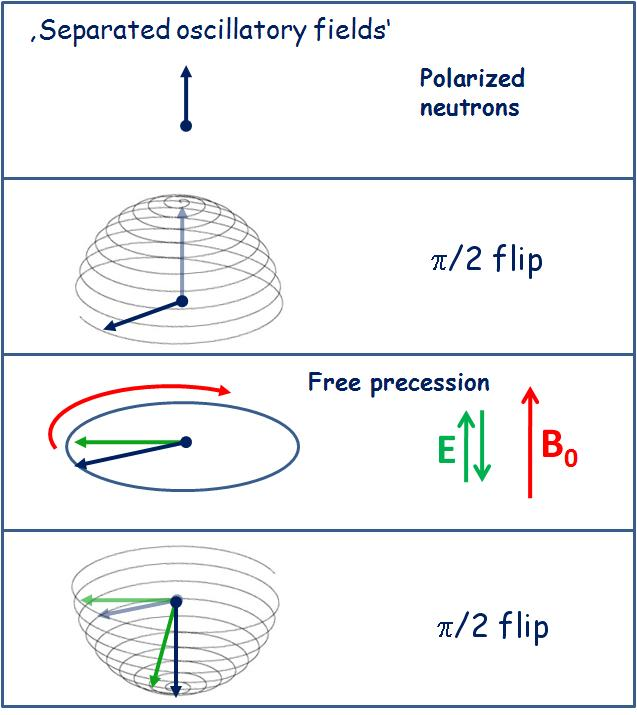
\includegraphics[width=0.4\textwidth]{images/ramsey.png}}
	\caption{Separated oscillatory fields from \cite{EDMReport}}
\end{figure}

As a measurement method the the commonly known method of separated oscillatory fields by Ramsey will be used. This is an interferometric nuclear magnetic resonance method applied to polarized and trapped ultra-cold neutrons. Spin polarized UCN precess in a highly homogeneous and constant magnetic field of 1$\mu T$. In an electric field applied along the magnetic field, a non-zero EDM would cause an additional level splitting, thus changing the Larmor frequency.\\


Ramsey's method of separated oscillatory fields: starting with an ensemble of polarized ultra-cold neutrons, the polarization is flipped into a precession plane normal to the constant field $B_{0}$. During a long period of free precession, an additional electric field E is applied parallel or anti-parallel to $B_{0}$, causing a small phase in the angle after precession. As the spin is flipped back along $B_{0}$, the deviation is analyzed. 

\section{Objectives}
The main target is to develop a prototypical implementation of a full functional data acquisition system. It should be possible to provide methods to insert data measured from devices. Those methods should be implemented in C/C++ and published through a library that supports Windows and Unix systems. Additionally a LabVIEW VI should be created that uses the functions to provide a template for upcoming implementations.\\
Furthermore, a user interface is required to visualize the stored data and to send commands to the measuring devices. Those commands or notifications should be received using event notification, especially active listening should be avoided. As a consequence to the data store that is going to be used, namely CouchDB, the user interface should be developed as a CouchApp. 		
		\chapter{Data Acquisition (DAQ)}
 
\section{Introduction}

In order to measure data from the experiment that can be analyzed, visualized and manipulated it is necessary to sample signals from sensors and convert them digital numeric values. This process is called data acquisition (DAQ) and can be achieved by various different software programs and a variety of general purpose programming languages. In general it can be differed in source, DAQ hardware and DAQ software. Whereas the source represents the sensor and measures the physical property, e.g. temperature, current, and magnetic flux density, DAQ hardware is usually the interface between the signal and the PC. Components like analog/digital converters, multiplexer, RAM etc. are common on this level. Microcontrollers, on which small programs run, can access those hardware devices via a bus and a protocol to make them available for further usage. DAQ software is necessary to make the DAQ hardware to communicate and work with a PC. While device drivers perform read and writes access at a very low-level on the hardware, standardized APIs \footnote{Application Programming Interfaces} enable a more abstract access and allow developing advanced user applications.\\

Data acquisition is an important part of the nEDM experiment since it is necessary to measure and store data from various sensors. Storing the data to make visualizing and analyzing possible afterwards is crucial to successfully run the experiment. There are lots of different aspects that need to be considered when setting up a new data acquisition system. To ensure a high quality system some basic requirements have to be met\cite{Schneider12, Marino12}:

\begin{itemize}
\item Expandability, to add a new subsystem
\item Adaptability, to handle different types of subsystems 
\item Security and Reliability, validation and backups to prevent data corruption
\item Layered Structure, to keep the system lucid and stable
\item Remote controllability, to have an easy access to the status of the experiment
\end{itemize}

\subsubsection*{Expandability}
Simple and modular implementation should lead to a system where new devices and subsystems are easily added. Adding additional devices should follow the "plug in and play" paradigm. No sophisticated implementation should be necessary when extending the system with new devices.

\subsubsection*{Adaptability}
Since subsystems can be implemented in a great variety of different controlling software and programming languages, e.g. LabVIEW, ORCA or python scripts, standardized interfaces are essential. Providing a fundamental application programming interface could meet this requirement and allows uncomplicated substitution of subsystems and devices. Furthermore adding devices to measure newly identified physical effects is getting easy.

\subsubsection*{Security and Reliability}
Encapsulation of used data storage should be possible. Different devices should be able to write on separate databases to avoid data loss or data corruption. Using this approach the risk decreases and different levels of accessibility can be set to prevent unauthorized access of the data. Furthermore continuous backup of all databases is required to prevent data loss caused by hardware failures or other errors. 

\subsubsection*{Layered Structure}
In software engineering the multi layer architecture is  common pattern to achieve logically separated functionality in a system. Functionality is implemented in independent modules that communicate with well defined interfaces. This very common model ensures a stable system, that is easy to understand and adapt. Data is stored on a database at the base layer. Separated from it a view/control layer is responsible to visualize and analyze the data.

\subsubsection*{Remote Controllability}
Watching the current experiments status should be possible and if necessary control devices from everywhere. Retrieving experimental data at a workstation in the laboratory, a PC at home or on a mobile device after authentication allows a remote access of the experiments status. Furthermore machine generated reports can automatically be send via mail to notify the project team of some extraordinary events or data.

\section{Data Acquisition Architecture}
\subsection{Multi-Tier Architectures}
A multi-tier architecture is common client-server architecture in which presentation, application processing, and data management funtions logically separated. Widely used thereby is the so called three-tier architecture. User interface, functional logic and data storage and access are developed and maintained as independent modules. This logical independence between the modules allows upgrades or changes without effecting the whole system. The usage of well-defined interfaces enables those separated evolve processes and therefore increases the agility and ability to meet upcoming requirements or changes.\\

Three-tier architectures consist of the following tiers:
 \begin{description}
     \item[Presentation tier] Visualizing data and interacting with the user are the most common services that are offered by the presentation tier. It retrieves data from the underlying data access tier and provides meaningful representations. This layer should furthermore be responsible for supplying user interfaces for devices accessing data, e.g. web browser at a PC or mobile device.
     \item[Application or data access tier] Data access tier is responsible for any business or data logic. Operations like selecting or aggregating data, as well as mathematical operations are performed within this layer. It expects data from the data tier and after executing necessary operations it serves the processed to the presentation tier according to the interfaces.
     \item[Data tier] This tier consists of the database storage. All data, that is measured by any sensor should be inserted and stored. Continuous backups as well as indexing and performance operations are kept at this level. The storage architecture itself should not be affected from any other tier.
  \end{description}
  
  
\begin{figure}[h!]
  \centering
      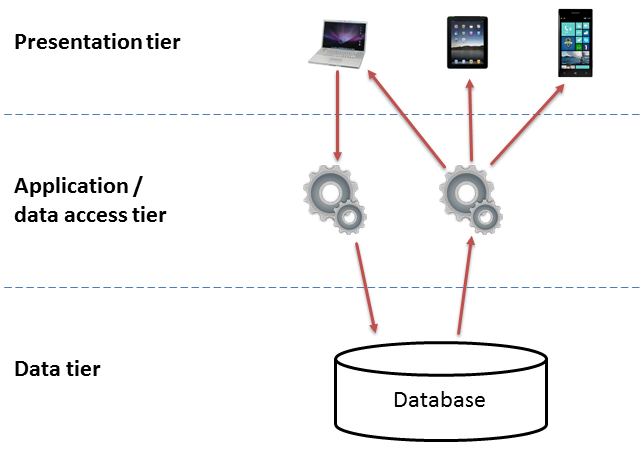
\includegraphics[width=0.7\textwidth]{images/3TierArchitecture.png}
  \caption{Schematic view of a three-tier architecture with one datastorage and different data representations using the data access level for information insertion and retrieval}
  \label{figure:3TierArchitecture}
\end{figure}

Figure \ref{figure:3TierArchitecture} shows an schematic overview of a three-tier architecture. A layer does only communicate with the tier that is directly below or above itself. The presentation layer does not call any functions from the database layer or vice versa.
  
\subsection{Data acquisition architecture at the nEDM experiment}
The three tier architecture is a very common pattern and used in many different software applications. Furthermore all patterns are best practices from a very abstract point of view. Therefore it is allowed to adapt this very general architectures to ones specific problem. Schneider showed the resulting architecture for the nEDM experiment in his bachelor thesis\cite{Schneider12}.\\

The architecture needs to provide three different layers to cover the requirements for the experiment. At the lowest level, there is a device layer that holds sensors measuring physical signals. Those signals are stored within a database, represented by a second layer. And the top layer is called View/Control layer and is responsible for providing views to the data and furthermore allows for controlling the database and physical devices via control parameters.
  
\begin{figure}[h!]
  \centering
      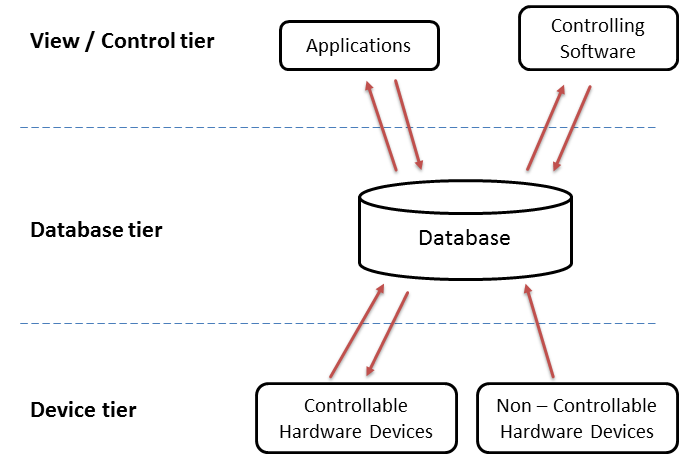
\includegraphics[width=0.7\textwidth]{images/DAQArchitecture.png}
  \caption{Adapted three tier architecture for the nEDM experiment}
  \label{figure:DAQArchitecture}
\end{figure}

Looking at the three tier architecture (see Figure \ref{figure:DAQArchitecture}) for the nEDM experiment more detailed, the following descriptions can be noted:
 \begin{description}
     \item[Device tier] The layer at the bottom is the hardware nearest layer. It consists of hardware controlling devices that are directly connected to all kinds of sensors. In general it can be differed between those sensors who can only send data to the database and those sensors that can furthermore also receive commands. 
     \item[Database tier] The database becomes the central part of the architecture. Beside its role as data storage it furthermore is responsible for the communication between the control applications and the hardware devices.  
     \item[View / Control tier] Although in standard three tier architectures the view layer is separated from the control layer, are those to tiers conflated to one. As we will see later on, the used technologies offer methods to combine the responsibilities of both layers. 
  \end{description}
  
  At this point a deviation from the standard pattern can be accepted because of the adaption to a very specific problem. Furthermore a best practice, recommended by National Instruments, encourages a design with four processes, that can be seen as tiers \cite{NI10}. Processes to handle GUI events, data acquisition and logging data is recommended. Furthermore they recommend a process to handle incoming messages from user interaction. The architecture used at the nEDM fulfills the guideline from National Instruments since all those tasks can be assigned to existing tiers. Whereas the handling of user interactions resides in the control tier. Beside of that National Instruments indicates that the proposed reference architecture is a "guideline that requires some customization to meet someones needs" \cite{NI10}.\\
  
After deciding, that CouchDB will be the database to store the experiments data, the architecture can be adapted to a concrete framework. Since all of the sensors, that are going to be used, need a PC or a small controlling device, they can communicate with the database with a program like LabVIEW, ORCA or scripts written in Python or C/C++ . The resulting framework for the data acquisition is according to the structure shown in Figure \ref{figure:ResultingFramework}. 
  
\begin{figure}[h!]
  \centering
      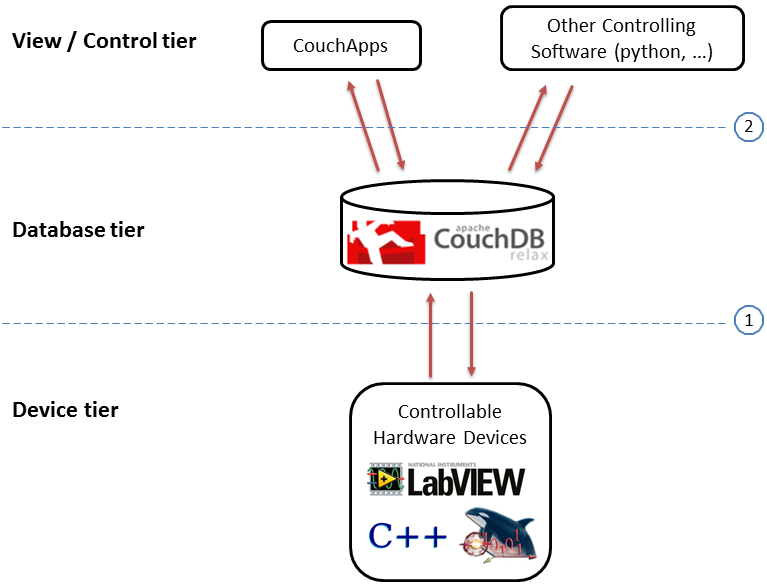
\includegraphics[width=0.7\textwidth]{images/ResultingFramework.png}
  \caption{Resulting framework for the nEDM experiment. Considering technical and conceptional aspects of necessary devices.}
  \label{figure:ResultingFramework}
\end{figure}

As shown in Figure \ref{figure:ResultingFramework}, the control and the device tier have to communicate with CouchDB. Therefore an API and a proper communication protocol has to be implemented. Two different interfaces exists regarding to the resulting framework:
\begin{itemize}
\item Between the device tier and the database tier (see Figure \ref{figure:ResultingFramework}: Interface 1)
\item Between the database tier and the view / control tier (see Figure \ref{figure:ResultingFramework}: Interface 2)
\end{itemize}
The communication between the view / control tier is easy, since so called CouchApps, small programs that are stored in the CouchDB and can access all data, are a built in functionality of CouchDB. They are mostly written in JavaScript and accessed via a web browser.\\
The interface between the device tier and the database is more sophisticated. Accessing CouchDB directly from LabVIEW is not possible and therefore an additional library is needed. This library is written in C (see Section \ref{section:implementation}). To ensure that this API allows different devices and sensors to send data to the database and receive data from it the functionality of the library has to be generic.

\subsection{Interfaces and communication between C and CouchDB}
Regarding to the resulting framework there exist two main interfaces (see Figure \ref{figure:ResultingFramework}). Whereas access the CouchDB via CouchApps is simple and easy to implement, accessing the database via C or C++ is not straightforward. Since it is possible to call C libraries from a LabVIEW solution, it is sufficient only to provide one platform independent library. Fortunately there is a platform independent library accessing CouchDB from any open-source project: pillowtalk \footnote{https://github.com/mgmarino/pillowtalk/}. This library uses libcurl and yajl to access CouchDB and communicates mainly via url targets. \\

\begin{figure}[h!]
  \centering
      \includegraphics[width=0.5\textwidth]{images/SendReceiveData.png}
  \caption{Bidirectional communication between hardware devices and the database}
  \label{figure:BidirectionalCommunication}
\end{figure}

Figure \ref{figure:BidirectionalCommunication} shows, that a bidirectional communication between the hardware devices should be possible. 
\begin{description}
     \item[Send Data] Every hardware device should be able to insert measured data into the database. This is crucial to every data acquisition system. An easy and generic way to insert is desirable. Different types of physical values are going to be stored. CouchDB is, unlike relational databases, document-based and without any given schema. Sending data, or data insert, is the basic operation and the pillowtalk library provides proper methods to perform the insertion of a new document. 
     \item[Receive Data] Hardware devices need be controllable. It should be possible to enable or disable them via the database or to send them commands to control their operations and set parameters. This functionality should be event based to avoid time and resource consuming polling tasks. 
\end{description}

To perform the bidirectional communication and to provide an interface to the functionality of pillowtalk a library called "AccCouchDB" \footnote{https://github.com/bwaltl/accCouchDB} was created. The library is platform independent and can be used on a Windows system or on Linux and Unix platforms. The library provides all functionality needed to insert data and to retrieve commands from the database. If a device wants to insert data, it is expected to register at the beginning at the database. This registration is necessary because later on, the CouchApp allows interaction only with registered devices. The registration process is quite easy since it consists only of one insertion with a fixed schema.

\begin{figure}[h!]
  \centering
      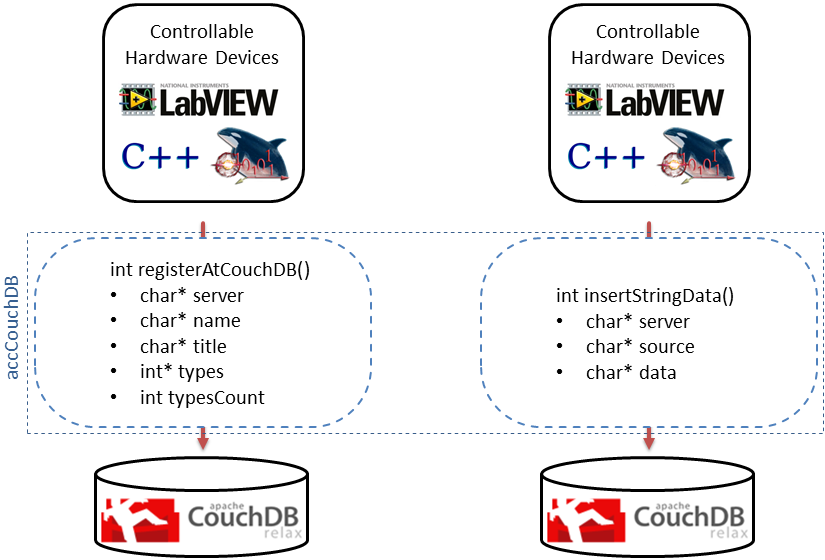
\includegraphics[width=0.7\textwidth]{images/SendingData2CouchDB.png}
  \caption{Inserting data at CouchDB}
  \label{figure:InsertingData}
\end{figure}

Figure \ref{figure:InsertingData} shows the two cases of a data insert operation. It is possible to register a device at CouchDB. This registration is done by calling a method named "registerAtCouchDB()":
\begin{description}
\item[char* server] The server parameter is used to connect to the database. It contains a string that holds the complete URL to the server and the database.
\item[char* name] The name parameter identifies the hardware device. This device name must be unique to ensure that it can be mapped correctly. 
\item[char* title] Since the name of a device must be unique within one database it is possible to define a more readable title to a hardware device. This must not be uniquely and allows a more detailed description of a device.
\item[int* types] A hardware device can be of a given type to enable aggregation or grouping at some view or controlling level. At the registration a device can specify to what types it belongs. Later on this could be mapped to, for instance, spatial or device type information.
\item[int typesCount] The number of types that a device belongs to. Length of the integer array "types".
\end{description}

Although it is not necessary, it may makes an implementation of a filter of notifications more convenient. This is more a preparation for further functionality, to develop some filtering functionality so that not every notification is passed to every device. \\

\begin{figure}[h!]
  \centering
      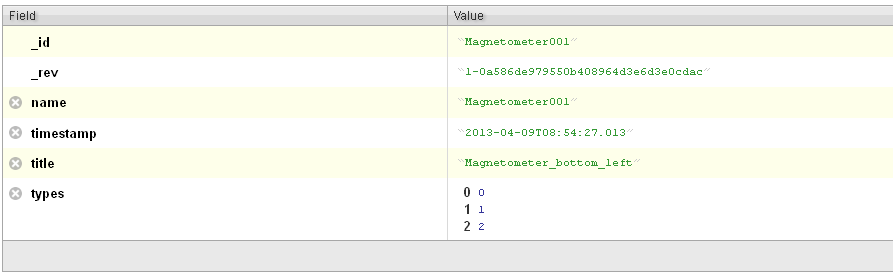
\includegraphics[width=0.9\textwidth]{images/CouchDBDoc_Register.png}
  \caption{CouchDB document format for a registered device}
  \label{figure:CouchDBDocumentFormat}
\end{figure}

Figure \ref{figure:CouchDBDocumentFormat} visualizes an inserted document at CouchDB. The id of the document is the name of the device, which is also contained in the "name" field. Also the "title" field is set to the value given by the function call. The types array contains three different values: 0,1,2. The "timestamp" field is set automatically by the accCouchDB library. \\

Figure \ref{figure:InsertingData} shows furthermore the data insert operation for measured data. This data insert is done calling the "insertStringData()":
\begin{description}
\item[char* server] The server parameter is used to connect to the database. It contains a string that holds the complete URL to the server and the database.
\item[char* source] The source parameter is used to map a data value to a device. The source string must match the "name" string that was specified by the registration of the device. 
\item[char* data] The data string contains the measured value of a physical phenomena. All data is stored as string values. 
\end{description}

Figure \ref{figure:CouchDBDocumentFormatData} shows an example of an inserted data document at CouchDB. The id of the document is the name of the device with a "data\_" prefix and an appended timestamp to ensure uniqueness. The "source" field is set to the value given by the function call that corresponds to the inserting device. The "data" field contains the measured value and the timestamp is added automatically.

\begin{figure}[h!]
  \centering
      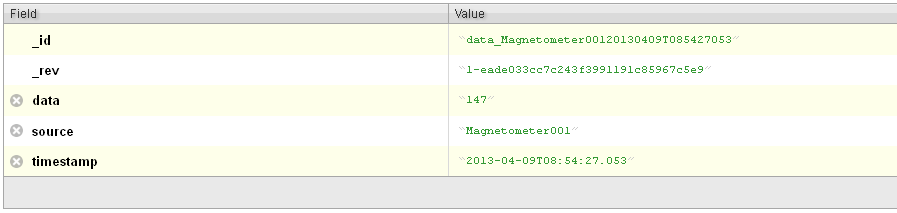
\includegraphics[width=0.9\textwidth]{images/CouchDBDoc_Data.png}
  \caption{CouchDB document format for measured data}
  \label{figure:CouchDBDocumentFormatData}
\end{figure}

\subsection{Retrieving commands and the CouchDB changes feed}
Enabling the possibility to turn on or off any functionality of the hardware device or to receive some other controlling commands it is necessary to communicate with the device. Since CouchDB supports notification services \footnote{http://guide.couchdb.org/draft/notifications.html} and the pillowtalk library also provides the functionality to use the changes feed it is not necessary for devices to poll if any commands are sent to them. Therefore there is a document type called "notification". \\

\begin{figure}[h!]
  \centering
      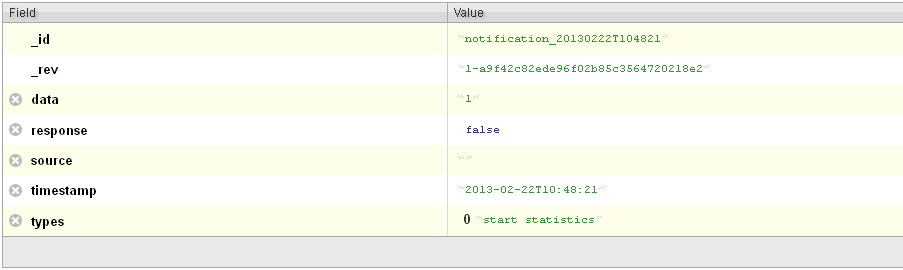
\includegraphics[width=0.9\textwidth]{images/CouchDBDoc_Notification.png}
  \caption{CouchDB document format for a notification}
  \label{figure:CouchDBDocumentFormatNotification}
\end{figure}

The notification document holds a data field of a value that is sent to the LabVIEW device. Furthermore it holds a response field that indicates if the transmission of the notification was successful. If not, the library creates a "error" field in the document in case of any error during the notification. This error field needs to be checked manually. It would be possible to implement further notification or logging in case of problems. Every command that will be sent to a device is stored in the database. Basically every controlling software is able to insert commands. \\

The notification is registered from the CouchDB with the changes feed functionality and is passed to LabVIEW using so called PostLVUserEvent \footnote{http://zone.ni.com/reference/en-XX/help/371361F-01/lvexcode/postlvuserevent/}. A LabVIEW VI can register to a changes feed of a CouchDB database and will be notified via callbacks on any changes or new documents. In principle only documents whose id field starts with "notification\_" will be passed. In more advanced applications additional filter methods will be required. This be implemented using the types field. To see how the notification process is implemented in LabVIEW see chapter \ref{section:implementation}.	
		\chapter{CouchDB}
\label{couchdb}
This chapter covers an introduction to \emph{Apache CouchDB}\footnote{\url{http://couchdb.apache.org}}. Thereafter,  For further information, see~\cite{Anderson10}.\\
CouchDB is a so-called \emph{NoSQL} database implemented in \emph{Erlang}\footnote{\url{http://www.erlang.org}}, whose aim is primarily facilitating horizontal scaling (distributed database). In contrast to common relational databases, it does not use tables to store data, but documents expressed in the \emph{JavaScript Object Notation} (JSON). Hence, a database in CouchDB consists of a set of documents. The advantage of store data as documents is simple extensibility and processing of the database.

\section{RESTful API}
\label{couchdb:restfulapi}
Since CouchDB provides a RESTful\footnote{\url{http://en.wikipedia.org/wiki/Restful}} API, and each of CouchDB's documents has its own, unique Uniform Resource Identifier (URI), every document can be retrieved and manipulated via the HTTP methods POST, GET, PUT and DELETE. Therefore, CouchDB basically also acts as web server, wherefore establishing a communication between CouchDB and a client is pretty straight-forward and simple.\\
Furthermore, CouchDB provides a web-based built-in administration interface called \emph{Futon}, supporting the creation, manipulation, and deletion of databases, views, and documents.

\section{Replication}
One of CouchDB's most famous features is \emph{replication}. This feature synchronizes two copies of the same database, allowing low latency access to data. Remarkably, this can also be done by appropriate HTTP methods. Therefore, creating backups of the database is a pretty simple task. Moreover, as stated later in chapter~\ref{couchapp}, since CouchApps are so-called \emph{Design documents}, which are in turn also common CouchDB documents, a backup of the database also applies to its CouchApps.

\section{Change Notifications}
\label{couchdb:changesfeed}
Another CouchDB feature is its \emph{changes feed}. By the use of this feature, applications can avoid polling of the database. In this context, polling refers to the repeated checking for changes in the database. However, in client-server scenarios, this may lead to a considerable increase of the network traffic.\\
Consequently, CouchDB's changes notifies all registered clients, when certain changes of documents occur, making polling unnecessary.

\section{Documents in CouchDB}
\label{couchdb:documents}
As already mentioned, a CouchDB database consists of a set of documents expressed in JSON. A document is self-containing, i.e. its schema information is contained in itself.\\
A CouchDB document might look like the following:
\begin{lstlisting}[language=json]
{
	"_id" : "albert_einstein",
	"_rev" : "1-dadc79bfe0af3d535d285d88b6e2df07",
	"Name" : "Albert Einstein",
	"Born" : 
	{
		"Year" : 1879, 
		"City" : "Ulm"
	},
	"Nobel Prize winner" : true,
	"Fields" : ["Physics"],
	"Address" : null
}
\end{lstlisting}
The attributes \emph{\_id} and \emph{\_rev} are both mandatory. The former has to be a unique key for the document, while the latter is the revision, which gets updated by each change of the document.\\
In addition to these mandatory attributes, each document may contain further attributes of one of the following types:
\begin{description}
\item[Number] An integer or even a decimal number. See the "Year" attribute of the example document.
\item[String] An arbitrary sequence of characters, enclosed by quotation marks. See the "Name" attribute of the example document.
\item[Boolean] Either \emph{true} or \emph{false}. See the "Nobel Prize winner" attribute of the example document
\item[Array] A sequence of arbitrary JSON objects enclosed by square brackets. See the "Fields" attribute of the example document.
\item[Object] A set of key-value-pairs enclosed by curly brackets, whereas the key has to be a string and the value can be of any of the listed types. See the "Born" attribute of the example document.
\item[null] Not a type, but represents an "empty value" or "nothing". See the "Address" attribute of the example document.
\end{description}
Furthermore, in CouchDB, documents can have attachments, i.e. arbitrary files (e.g. *.html and *.js files) can be attached to documents. These attachments get their own URL by which they are accessible and manipulable.

\section{Querying CouchDB}
\label{couchdb:query}
While in relational databases, data sets are queried and manipulated by the Structured Query Language (SQL), CouchDB uses so-called \emph{map} and \emph{reduce} functions, known as MapReduce.\\
The map function is invoked for each of the source's documents. Because of the independence of these function applications, this can be done in parallel enabling horizontal scaling. Map functions can emit an arbitrary number of key-value-pairs, hence, the may, for example sort out certain documents to implement a filter operator.\\
All key-value-pairs emitted by the map functions are distributed into certain groups, which are determined by their keys, i.e. all key-value-pairs with the same key are allocated to the same group. Subsequently, the reduce function is called once for each group with each group as its argument. This can also be done independently and in parallel.\\
In CouchDB, a combination of map and reduce function is called \emph{view}. Figure~\ref{img:mapreduce} shows an exemplary definition of a view, grouping a list of scientists (documents) by their scientific field (in the map function) and counting the scientists per field (in the reduce function).
\begin{figure}[h!]
\centering
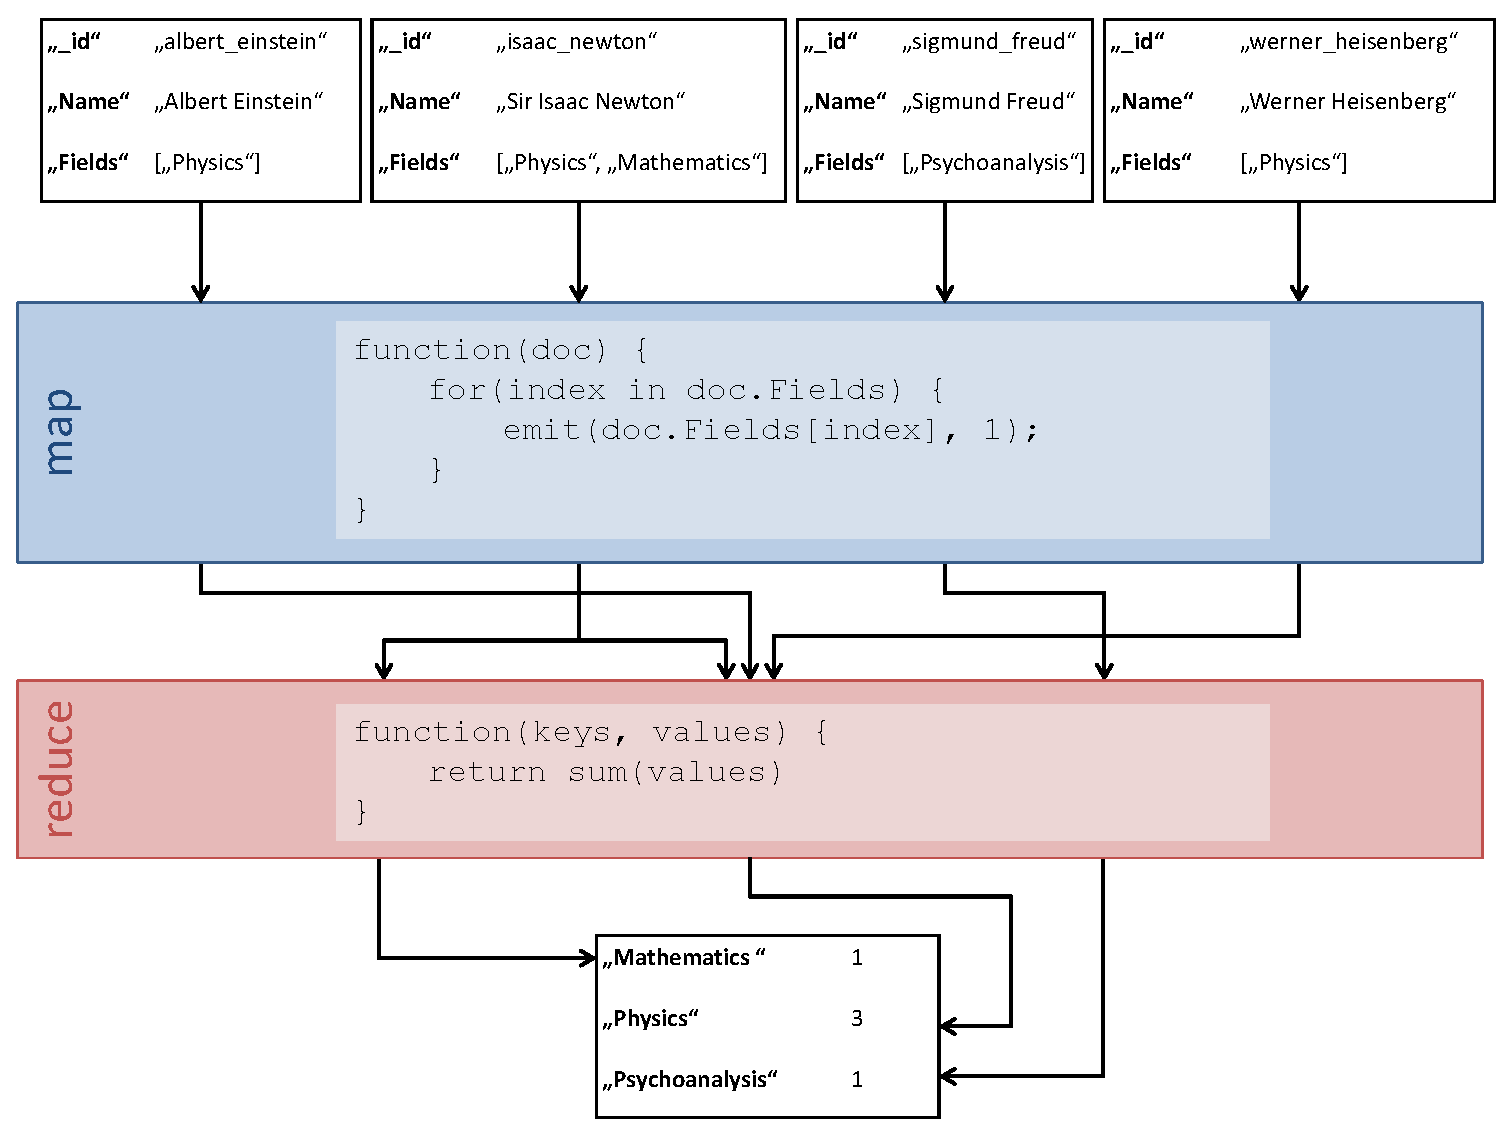
\includegraphics[width=1.0\columnwidth]{images/mapreduce.pdf}
\caption{Definition of a view by MapReduce to count the scientists per field}
\label{img:mapreduce}
\end{figure}

\section{Design documents}
\label{designdocument}
Queries can be either temporary or they can be stored to the database, whereas a query is stores as a \emph{Design document}, having an attribute "views", which contains the map as well as the reduce function (see Figure~\ref{img:couchdbviewdocument}). In Futon, stored views can be selected in the database view as shown in Figure~\ref{img:couchdbviewselection}.\\
\begin{figure}[h!]
\centering
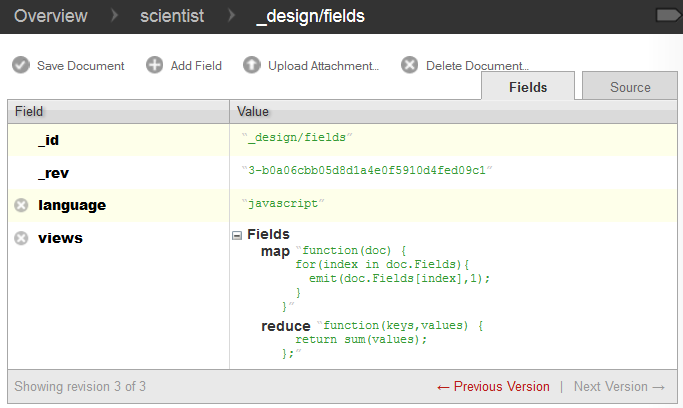
\includegraphics[width=0.65\columnwidth]{images/couchdbviewdocument.png}
\caption{A CouchDB view as a Design document}
\label{img:couchdbviewdocument}
\end{figure}

\begin{figure}[h!]
\centering
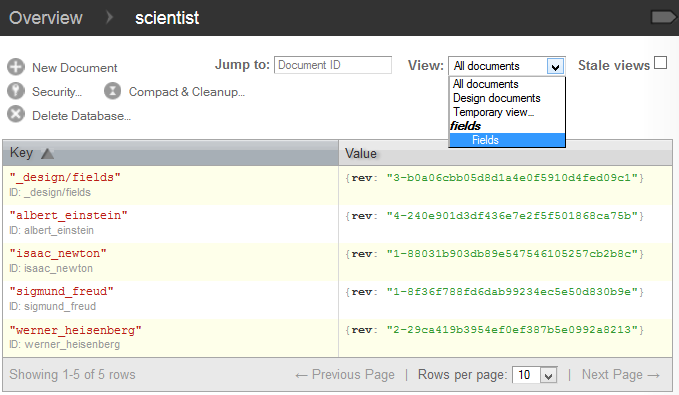
\includegraphics[width=0.65\columnwidth]{images/couchdbviewselection.png}
\caption{Selection of the stored view "Fields" in CouchDB's Futon}
\label{img:couchdbviewselection}
\end{figure}

Design documents are basically common CouchDB documents, however, they may have a special purpose for the CouchDB. This means, although they are stored like common data, they fulfill special roles, e.g. defining queries (as mentioned in the previous Section) or defining CouchApps (see Chapter\~ref{couchapp}). To differentiate common documents from Design documents, the value of each Design document's \emph{\_id} attribute starts with the "\_design\/" prefix.

		\chapter{Data Acquisition using LabVIEW}

\section{Introduction}
The graphical programming environment LabVIEW \footnote{Laboratory Virtual Instrumentation Engineering Workbench, see http://www.ni.com/labview/} includes a variety of hardware drivers to allow the usage of many different hardware devices. Furthermore LabVIEW is commonly used in data acquisition and instrument control. Platform independent hardware access is an additional benefit of the LabVIEW components. Since it is a graphical environment where the programs and routines are developed and there are lots examples included creating small applications is simple. The modular character of LabVIEW programs allows code reuse without modifications. LabVIEW contains an extra compiler that produces native code for the CPU platform. Therefore it is platform independent and developed programs can easily be deployed on different operating systems like Windows, Mac OS X and Linux. The LabVIEW version used to develop the data acquisition modules was LabVIEW 2011 SP1 (release date 1 March 2012).

\section{Requirements}
The slow control acquisition system collects a variety of different parameters from the experiment, e.g. magnetic field values, vacuum quality, temperature, etc. Additionally it should be possible not only to measure, store and analyze data, furthermore it should be capable of controlling devices. Enable or disable the vacuum pump, open or close valves, etc. To achieve this, there has to be a mechanism that allows the control system to send commands to the devices. Afterwards those commands are processed by the devices.\\

The slow control acquisition handles a slow and permanent submitted data flow. The system should be able to process a data stream with about one data value per second and device. That is way it is called slow control. Beside this data acquisition there is also a fast data acquisition that is not part of this project.\\

The data is stored in a CouchDB database. An access should be possible using so called CouchApps. A big advantage is that those are stored directly in the database and provide a platform independent access since they are mainly written in JavaScript and therefore accessibly through a web browser.\\

The hardware devices should be controllable via short commands that are sent using the database. After inserting such a command, the device should be notified and receive the command instantly. To perform this, it registers to a notification service. Active listening should be avoided.\\

The main part consists of providing a library that handles the interaction and communication with the CouchDB. It provides methods to insert and receive data. Preferably, the library should be platform independent since different operating systems are required to run the experiment properly.\\

\section{Implementation}
\label{section:implementation}
The implementation part of the data acquisition system consists of two different interfaces and the LabVIEW projects. In this chapter the interface 1 from figure \ref{figure:ResultingFramework} as well as the C - library at the device tier are going to be discussed and described in more detail. 

\subsection{LabVIEW VI}
LabVIEW implementations are organized in so-called virtual instruments and represent the programs. In this implementation a VI was developed to show the basic functionality and to fulfill the requirements (insert data and retrieve notifications). A VI consists of two different interfaces. A front panel and a block diagram. The front panel is used for user interaction and to visualize and display information to the user and the block diagram contains the graphical source code. 

\subsubsection{Calling an external function in LabVIEW}
\label{section:callingExtFunction}
To call an external function in LabVIEW a block diagram node called Code Interface Node (CIN) is used \cite{ExtCodeLabView} (see Figure \ref{figure:CIN}a). 
 \begin{figure}[h!]
   \centering
%   \subfiguretopcaptrue
    \subfigure[]
    {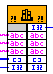
\includegraphics[width=.08\textwidth]{images/CIN.png} \hspace{0.2cm}}
     \subfigure[]
    {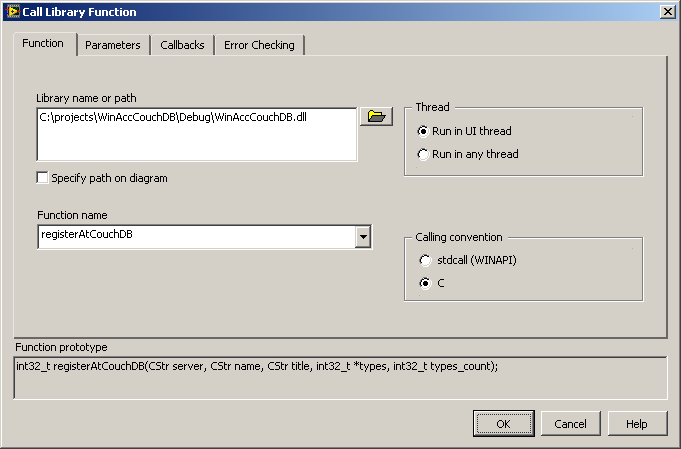
\includegraphics[width=.4\textwidth]{images/CINDetails1.png}\hspace{0.2cm}}
    \subfigure[]
    {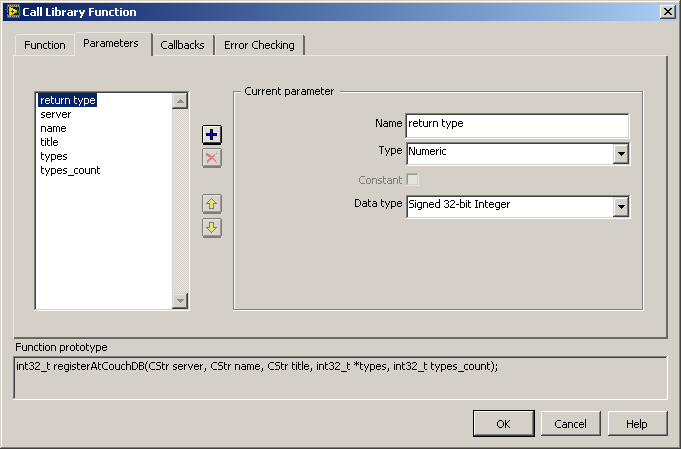
\includegraphics[width=.4\textwidth]{images/CINDetails2.png}}
     \caption{The Code Interface Node and its properties dialog}
     \label{figure:CIN}
  \end{figure}

The CIN can be configured to call a specific function of a C - library. The library can be a Windows library *.dll or a Linux shared object *.so. Within LabVIEW the path to the library is required and additional the header file is necessary to get the parameter lists and functions that are provided by the library. The CIN provides an separate input for every parameter that is expected from the function. Furthermore all inputs need to be connected to some value providing method. This properties can be set in the properties dialog from the CIN. Figure \ref{figure:CIN}a) and b) show the two important tabs of CIN properties. At b) the path to the library and the header file is set. It is also possible to set the calling convention and to the set executing thread. This should be set to the default values. The second tab allows to set the parameters that are necessary to call the function. It is able to set the name, the data type and an option to specify whether it is an array or some numerical value. It is recommended to import a library via the built in function of LabVIEW. The wizard can be found in the menu Tools$\rightarrow$Import$\rightarrow$shared library (.dll) (see Figure \ref{figure:ImportWizard}). The CINs are created automatically and the parameters and return values are set properly\footnote{There is a bug under Windows: if the wizard tries to import a library function that requires some data type from the LabVIEW library "extcode.h". This is the case for the function "InitChangesFeed()". In this case the parameters have to be set manually, whereas the type of the UserEventRef needs to be set to "Adapt to Type".}. To enable a correct import and to call the C - library functions it must be ensured that all libraries that are required can be found. To ensure this, copy all necessary libraries (yajl, libcurl, pillowtalk and in case of Windows pthreadVSE2) in the same folder as the accCouchDB library.

\begin{figure}[h!]
	\centering
		\subfigure[]
      		{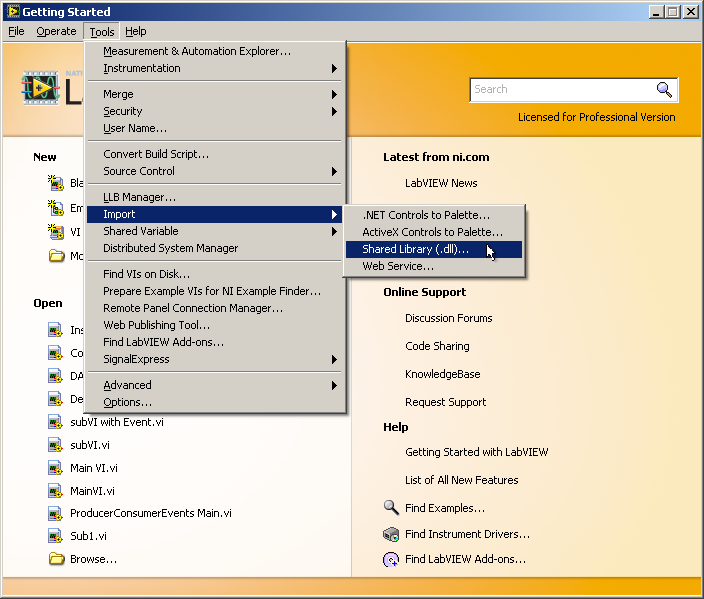
\includegraphics[width=0.4\textwidth]{images/ImportWizard.png}\hspace{1.0cm}}
		\subfigure[]
			{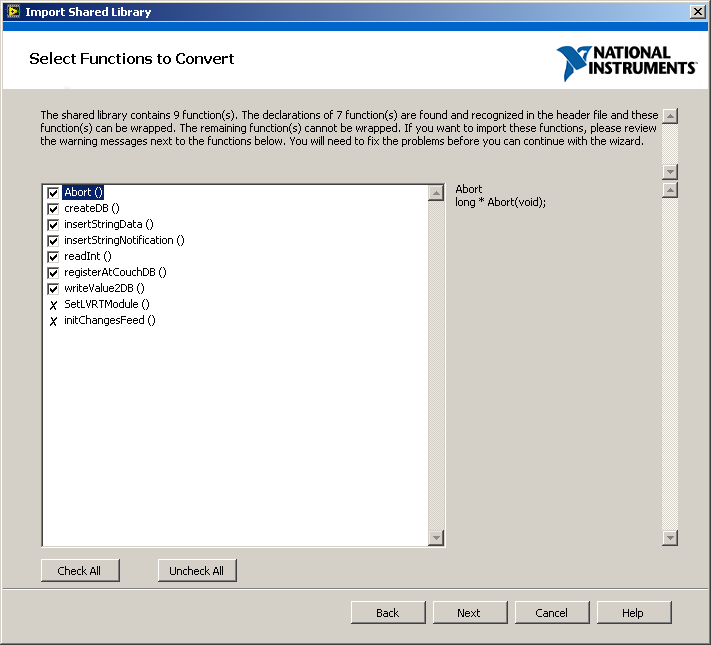
\includegraphics[width=0.4\textwidth]{images/ImportWizard2.png}}
	\caption{Import wizard for shared libraries in LabVIEW}
	\label{figure:ImportWizard}
\end{figure}

\subsubsection{Inserting data and registration of a device}
 
\begin{figure}[h!]
  \centering
      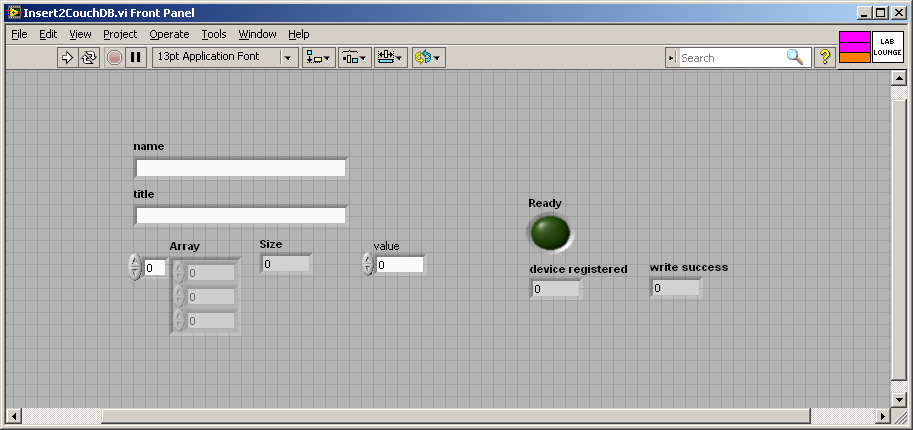
\includegraphics[width=0.9\textwidth]{images/InsertValue2CouchDBfront.png}
  \caption{Front panel of the LabVIEW VI used to register a device and insert a data value.}
  \label{figure:InsertValue2CouchDBfront}
\end{figure}

Figure \ref{figure:InsertValue2CouchDBfront} shows the front panel for a VI that can be used to register a device at the CouchDB and insert a data value. In the front panel the user can specify the name and the title for the device, furthermore an array of numbers can be created to specify the types for one device. After filling the input form the VI can be executed by pressing the "run" button. The program will be executed once and the return values are displayed in the front panel. Figure \ref{figure:InsertValue2CouchDBfrontDone} shows the front panel after the successful execution of the VI. 

\begin{figure}[h!]
  \centering
      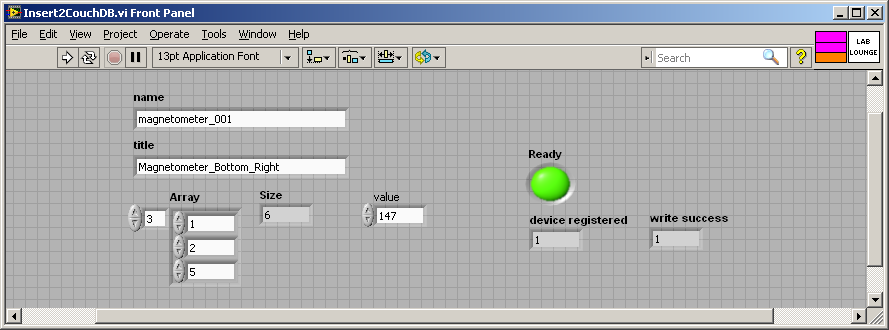
\includegraphics[width=0.9\textwidth]{images/InsertValue2CouchDBfront_done2.png}
  \caption{A VI after a successful device registration and data insertion.}
  \label{figure:InsertValue2CouchDBfrontDone}
\end{figure}

The successful execution can be seen at the two return values. The "device registered" and the "write success" return values are both set to one, which indicates the completion without errors.\\

To see the actual program one have to look at the block diagram. The block diagram consists of the program blocks and represent the functionality of the VI. 

\begin{figure}[h!]
  \centering
      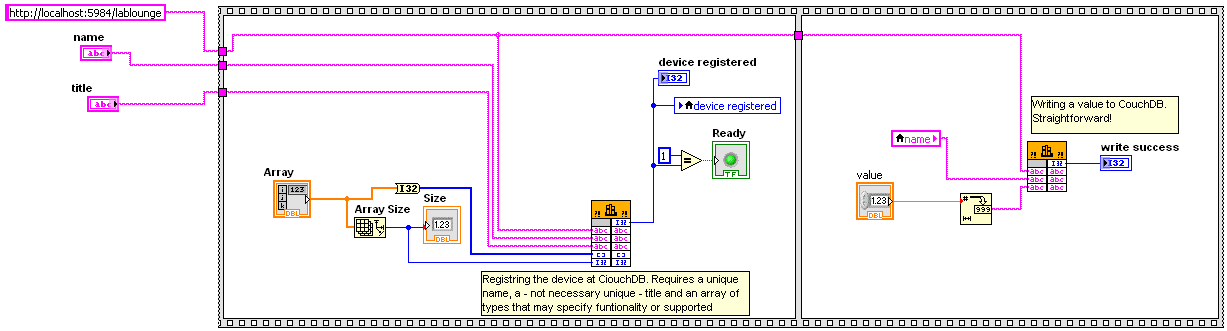
\includegraphics[width=0.9\textwidth]{images/InsertValue2CouchDB.png}
  \caption{The block diagram of the VI.}
  \label{figure:InsertValue2CouchDB}
\end{figure}

The program itself (shown in Figure \ref{figure:InsertValue2CouchDB}) is quite simple. There are only a few methods required to ensure the registration and the insertion of a data value. In principle it consists of two different functions. In the left part of the grey box the device registration is done and afterwards a data value is inserted. The database location is set as a constant. The most important parts are the methods to call an external C function. Those methods require several input parameters and return a value representing the success of the method. The registration in the left part of the grey box needs the location of the database as well as the name and the title of the device. Furthermore an array of numbers can be passed. The result is a number which is displayed in the front panel of the VI (see Figures \ref{figure:InsertValue2CouchDBfront} and \ref{figure:InsertValue2CouchDBfrontDone}). The right part of the grey box handles the insertion of the data value. It requires only the database location and the name of the device and of course the data value, that is going to be stored. The return value is displayed in the "write success" field afterwards. The grey box is a control structure that ensures that the device is registered before it inserts data. The program blocks are executed one after another, beginning with the leftmost block.

\subsubsection{Retrieving notifications from CouchDB}
 
\begin{figure}[h!]
  \centering
      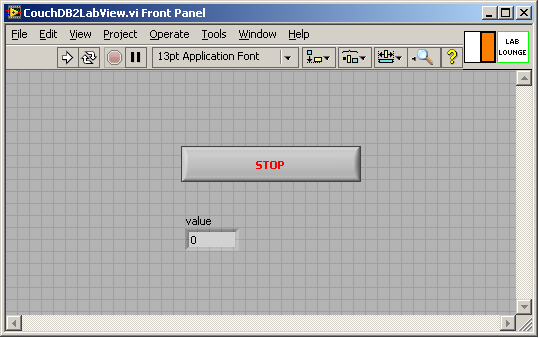
\includegraphics[width=0.4\textwidth]{images/CouchDB2LabVIEWFront.png}
  \caption{Front panel of the LabVIEW VI used to retrieve data values from CouchDB.}
  \label{figure:CouchDB2LabVIEWFront}
\end{figure}

The front panel structure of the VI to retrieve notifications from CouchDB is very simple. It consists of an number indicator to visualize the command that was retrieved and a button to stop the execution and especially the listening thread. 

\begin{figure}[h!]
  \centering
      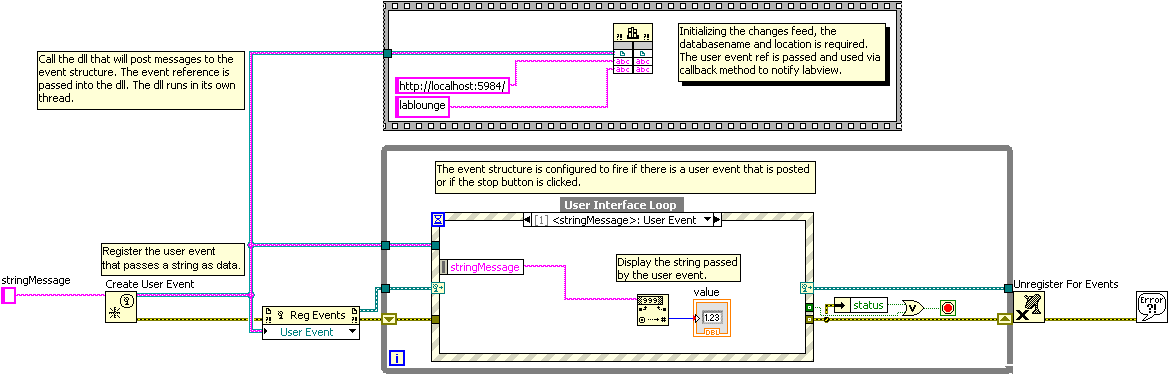
\includegraphics[width=0.9\textwidth]{images/CouchDB2LabVIEW.png}
  \caption{Block diagram of the LabVIEW VI used to retrieve data values from CouchDB.}
  \label{figure:CouchDB2LabVIEW}
\end{figure}

The block diagram (shown in Figure \ref{figure:CouchDB2LabVIEW}) is more sophisticated. It mainly consists of two different execution parts. The upper part is to initialize the thread at the C library. The method requires the location of the database as well as the database name. Furthermore a UserEventReference object is required. This object is created with the function at the very left and used to call the callback function. The UserEventReference is instantiated with an string object as input parameter. As a consequence a string object is expected as parameter in the callback function. The C library is casting every command, that will be sent to LabVIEW, to a string value. The UserEventReference is registered and handled within "User Interface Loop" which handles all events that are generated by the UserEventReference object. Whenever the object fires an event, the content of the stringMessage variable will be read and displayed to the user. The variable could also be read from any other method. Since functions run parallel in LabVIEW changing the stringMessage value causes a VI wide change, so that the change can be seen from everywhere in the VI.\\
\begin{figure}[h!]
  \centering
      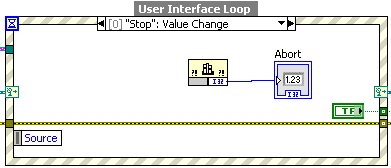
\includegraphics[width=0.5\textwidth]{images/CouchDB2LabVIEW_stop.png}
  \caption{Pressing the stop button terminates the listener thread and the VI.}
  \label{figure:CouchDB2LabVIEWstop}
\end{figure}
The "User Interface Loop" also handles the stop button (see Figure \ref{figure:CouchDB2LabVIEWstop}). If it is pressed by the user the C - library function "Abort" is called an the execution of the thread terminates. This should be done whenever the VI is going to be stopped to ensure that the threads are closed properly and allocated memory is freed. The execution would also stop if there is some error while registering the UserEventReference.

\subsection{C - Library}
The library is accessible on github\footnote{https://github.com/bwaltl}. There are three different repositories available:
 \begin{description}
     \item[accCouchDB] This repository runs on Unix and Windows systems. It provides cross platform compilation using cmake. Additionally it provides all libraries that are necessary to compile under MS Windows. Should be used for further development!
     \item[WinAccCouchDB] This repository is a full Visual Studio 2008 project that produces a version of AccCouchDB library that runs on all Windows systems. 
     \item[UnixAccCouchDB] The Unix version that was created with Eclipse\footnote{http://www.eclipse.org/} and a C/C++ plugin. It produces an shared object library that can be used on Unix systems.
  \end{description}
  
It is recommended to use the cross platform version \textit{accCouchDB}\footnote{https://github.com/bwaltl/accCouchDB} to ensure that changes are made on both, the Unix and MS Windows, versions of the library.

\subsubsection{Building the library}
The library depends on three different other libraries that need to be installed (Unix systems) or otherwise accessible. Anyway they are required to build the AccCouchDB library. 

 \begin{description}
     \item[yajl\footnote{http://lloyd.github.io/yajl/}] A JSON library used to create JSON objects. Necessary to create the communication objects.
     \item[libcurl\footnote{http://curl.haxx.se/libcurl/}] The file transfer protocol library \textit{libcurl} is used to communicate with the CouchDB using URLs. 
     \item[pillowtalk\footnote{https://github.com/mgmarino/pillowtalk/}] ANSI C library that talks to CouchDB using libcurl and yajl.
     \item[pthreadVSE2 (only MS Windows)] On Windows systems an additional threading library is required. Should be available by default. 
  \end{description}
  
Since building these libraries can cause troubles, they are available in the github repositories. In general they should work without great problems, otherwise they have to be created manually following the building instructions of the affected library. \\

After creating a local clone of the AccCouchDB it can be build using the makefile. It is necessary to update the library paths in the \textit{CMakeLists.txt} file that is stored in the \textit{.../AccCouchDB/src/} folder. \\

In MS Windows systems it is sufficient to install the Visual Studio 2008 to ensure that the compiler is available and afterwards start the \textit{Visual Studio 2008 Command Prompt}. To see if the compiler is correctly installed type:\\
\shellcmd{cl}\\
Switch to the folder of the AccCouchDB project and create a build folder:\\
\shellcmd{mkdir build}\\
\shellcmd{cd build}\\
Start the build process by executing the following command:\\
\shellcmd{cmake -G"NMake Makefiles" "..$\backslash$src$\backslash$"}\\
Afterwards the library can be created using the makefile:\\
\shellcmd{nmake}\\
If every step was successfully executed there should be a \textit{AccCouchDB.dll} in the build folder of the project. The corresponding header file \textit{AccCouchDB.h} is in the source folder of the project.\\

In Unix systems it is sufficient to make sure that the gcc compiler is available. To see if the compiler is correctly installed type:\\
\shellcmd{gcc}\\
Switch to the folder of the AccCouchDB project and create a build folder:\\
\shellcmd{mkdir build}\\
\shellcmd{cd build}\\
Start the build process by executing the following command:\\
\shellcmd{cmake "..$\backslash$src$\backslash$"}\\
Afterwards the library can be created using the created makefile:\\
\shellcmd{make}\\
If every step was successfully executed there should be a \textit{AccCouchDB.so} in the build folder of the project. The corresponding header file \textit{AccCouchDB.h} is in the source folder of the project.\\

Beside of all those libraries it is required, that LabVIEW is installed on the operating system. To enable the callback functionality the LabVIEW library \textit{labview.dll} is required. \\
The library file \textit{AccCouchDB.dll} can be used in LabView to communicate with the CouchDB. See chapter \ref{section:callingExtFunction} for more details.

\subsubsection{Functions and implementation}
The C library contains functions, that enable the communication with the CouchDB in a bidirectional way. Basically two things are possible: On the one hand inserting and persisting measured data and on the other hand retrieving notification commands from CouchDB.\\

Inserting data is quite easy and straightforward. This is achieved by calling the function "insertStringData(...)". The function consists mainly of two things, that need to be performed. At the beginning the document has to be created and the proper attributes have to be filled with data. 
\begin{lstlisting}[language=C++]
//create a new document
pt_node_t* root = pt_map_new();

//set the device, that inserts the data
pt_map_set(root, "source", pt_string_new(source));

//retrieve a timestamp
string timestamp = getTimestamp();
pt_map_set(root, "timestamp", pt_string_new(timestamp.c_str()));

//set the data value
pt_map_set(root, "data", pt_string_new(data));
	
//create a unique id 
string id = "data_" + string(source) + getTimestampasID();
pt_map_set(root, "_id", pt_string_new(id.c_str()));
\end{lstlisting}

And the second part of the function is to save the document at CouchDB by calling the \textit{pt\_put(...)} function from pillowtalk.
\begin{lstlisting}[language=C++]
pt_response_t* response = NULL;

//try to insert the document
response = pt_put(keyPath.c_str(), root);
if (response->response_code != 201) {
	log_stringMessage("Data insertion failed", keyPath.c_str());
	log_intMessage("Data insertion failed", response->response_code);
	return OPERATION_FAILED;
}
return OPERATION_SUCCEDED;
\end{lstlisting}

Retrieving notifications from CouchDB can be initialized calling the \textit{initChangesFeed(...)} function. It expects a user reference object, that is stored to call the LabVIEW VI in the callback function.

\begin{lstlisting}[language=C++]
rwer = local_rwer; // store the UserEventRef object

// initialize the changes feed + heartbeat function 
pt_changes_feed_config(cf, pt_changes_feed_continuous, 1);
pt_changes_feed_config(cf, pt_changes_feed_req_heartbeats, 1000);

// register the callback function
pt_changes_feed_config(cf, pt_changes_feed_callback_function, &callback);
pt_changes_feed_run(cf, server, database);
\end{lstlisting}

If an event raises the callback function is called and the most important part there is calling the \textit{PostLVUserEvent(...)} method that is provided by LabVIEW. It requires the UserEventReference object and a string handle object that holds the value that is passed to labview.

\begin{lstlisting}[language=C++]
MgErr result = PostLVUserEvent(*rwer, (void *) &newStringHandle);
\end{lstlisting}

If the execution of a VI stops, the function \textit{abort()} should be called to ensure that the notification threads are halted.\\

Furthermore the library contains more functions to allow different operations. Some of them are useful for development. It is possible to enable or disable logging of the library. Or to create a new database or to insert single data values to a document or read values from a document with a given key. Most of the functions are straightforward and easy to understand. A recommended function that is very useful during the development process is the function \textit{DebugPrintf(...)\footnote{http://zone.ni.com/reference/en-XX/help/371361G-01/lvexcodeconcepts/debugging\_external\_code/}} provided by LabVIEW. It displays string values in a debugging console of LabVIEW and offers a good way to find bugs or other strange behavior in the library functions.

\subsection{A prototypical VI using NI USB-6211}
To combine all the functionality in LabVIEW and to prove the performance of the C library an existing VI was extended to the usage of the DAQ concept of the nEDM. The VI measures a magnetic field and displays the offset and the standard deviation. Those values are logged in a file. The VI was extended to write the value to the CouchDB and to enable or disable the logging function via notification commands sent from CouchDB. \\

\begin{figure}[h!]
  \centering
      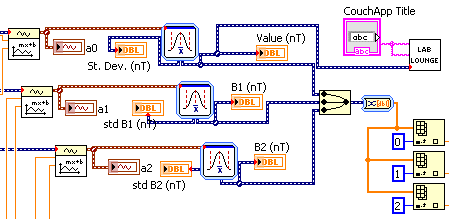
\includegraphics[width=0.4\textwidth]{images/VIExample.png}
  \caption{The insert functionality is encapsulated in a SubVI and only requires a sensor name and the value.}
  \label{figure:ExampleVI}
\end{figure}

Figure \ref{figure:ExampleVI} shows how the functionality can be implemented to an existing VI. The SubVI can be opened by double-clicking on the symbol. The \"CouchApp Title\" is set in the front end of LabVIEW and represents both, the name and the title of the sensor. \\

\begin{figure}[h!]
  \centering
      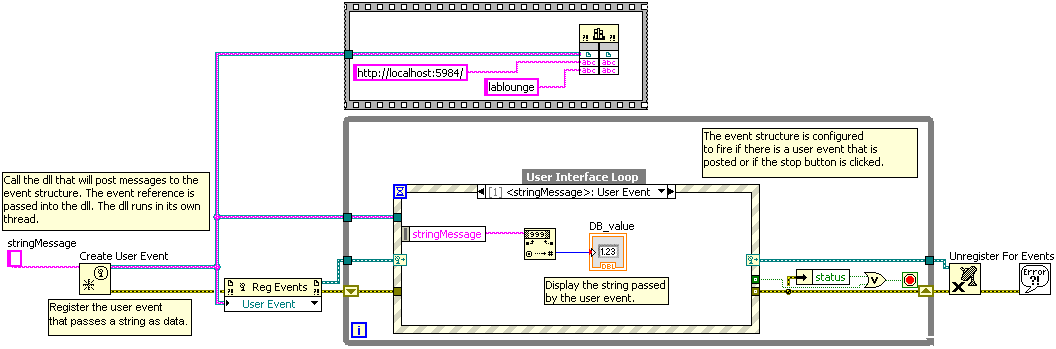
\includegraphics[width=0.9\textwidth]{images/VIExample_notification2.png}
  \caption{Receiving notifications and storing values in a local variable.}
  \label{figure:ExampleVI_receiving}
\end{figure}

Figure \ref{figure:ExampleVI_receiving} represents the functionality of receiving notifications from the CouchDB. After the initialization the event structure is called in case of an event. Afterwards the value that was received is stored in a local variable. \\

\begin{figure}[h!]
  \centering
      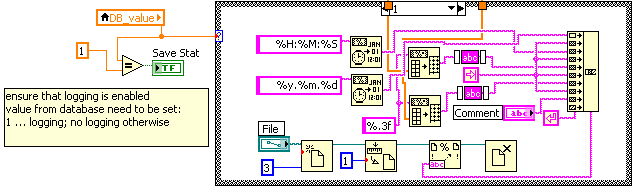
\includegraphics[width=0.5\textwidth]{images/VIExample_notification.png}
  \caption{Logging depends on the value sent from the CouchDB.}
  \label{figure:ExampleVI_receiving}
\end{figure}

Figure \ref{figure:ExampleVI_receiving} shows the VIs logging functionality. If the value of \textit{DB\_value} is set to zero the logging process is no longer executed and therefore no values are stored in a local file.  \\
		\lstset{language=HTML}

\chapter{CouchApp}
\label{couchapp}
As already mentioned in Section~\ref{couchdb:restfulapi}, CouchDB also acts as web server, i.e. it provides resources (its documents), which are accessible via the web by using HTTP methods. Furthermore, CouchDB provides an integrated JavaScript web application framework called \emph{CouchApp}.\\
CouchApps are stored as common documents, or more precisely, \emph{design documents}. Hence, they are easy to edit and share, and are even replicable like other documents. However, this design documents have a lot of attachments, e.g. HTML and JavaScript files, images, CSS style sheets, etc.
\section{Developing CouchApps}
\label{couchapp:development}
To support the development and deployment of CouchApps, you can download and use the CouchApp tool\footnote{\url{http://couchapp.org}}. This tool prepares an appropriate CouchApp project structure on the one hand, and provides tool-supported deployment of the CouchApp on the other hand.\\
Moreover, we strongly recommend the use of a HTML and JavaScript editor providing syntax highlighting and auto completion, e.g. Microsoft's Visual Studio\footnote{\url{www.microsoft.com/visualstudio}}. For this purpose we created a CouchApp project template for Visual Studio 2012, which integrates the CouchApp tool and thus offers an Integrated Development Environment (IDE) for the development of CouchApps.\\
To deploy the project template in Visual Studio 2012, you just have to copy the template file "couch App.zip" into the project templates folder of Visual Studio (in windows operating systems: "<user>/Documents/Visual Studio 2012/Templates/ProjectTemplates). Consequently, in the "New Project" dialog of Visual Studio, the CouchApp template should appear, as shown in Figure~\ref{img:vsprojecttemplate}.
\begin{figure}[t!]
\centering
\includegraphics[width=0.75\columnwidth]{images/VSprojecttemplate.png}
\caption{CouchDB project template in Visual Studio}
\label{img:vsprojecttemplate}
\end{figure}
To ensure a faultless development of CouchApps with Visual Studio 2012, make sure to encode all files with UTF-8 (without signature) as shown in Figure~\ref{img:vsfileencoding}.

\begin{figure}[t!]
\centering
\includegraphics[width=0.50\columnwidth]{images/VSfileencoding.png}
\caption{Select "UTF-8 without signature" as encoding for all files in the CouchApp}
\label{img:vsfileencoding}
\end{figure}

A CouchApp project contains the following folders and files:
\begin{description}
\item[.couchappignore] Defines files or folders, which may be located inside the CouchApp directory, but should not be deployed to the CouchDB
\item[.couchapprc] May contain several deployment configurations, e.g. location of the CouchDB, authentication data, ...
\item[couchapp.json] Contains basic information about the CouchApp, e.g. its name, a short description, ...
\item[\_id] Contains the ID of the design document
\item[README.md] May provide some information about the CouchApp and how to access it
\item[\_attachments/] This folder contains the CouchApp's layout (index.html), CSS style sheets and some other files. These files will be deployed as attachments of the design document.
\item[vendor/] The files in this folder are usually from other sources, e.g. jQuery, jQuery UI, etc. These files will also be deployed as attachments of the design document.
\item[views/] May contain some predefined CouchDB views consisting of a map and an optional reduce function (as introduced in Section~\ref{couchdb:query}).
\end{description}
\section{Introduction to Evently}
\label{couchapp:evently}
Another very important folder in a CouchApp is "evently", which is containing folders and files belonging to the Evently jQuery plugin\footnote{\url{http://couchapp.org/page/evently}}. Evently empowers the developer to extend the set of common standard client-side web events (clicks, changes in text boxes, moving the mouse over a user control, ...) by more concrete custom events (selection of a specific device, submission of a new notification, ...).\\
Standard events are usually triggered by single elements of a browser's Document Object Model (DOM), e.g. a single button is clicked, the text in a text box has changed, the mouse enters the area of a div, a option in a drop-down list is selected, etc. These events can be handled by so-called event handlers, which are normally functions with the following two parameters:
\begin{description}
\item[sender] The sender parameter is the object, which triggered the event (e.g. the button which was clicked)
\item[args] This parameter may contain event-specific information (e.g. the selected option in a drop-down list)
\end{description}
\subsection{Evently Widgets}
\label{couchapp:evently:widgets}
While standard events are triggered by common DOM elements, Evently's custom events are triggered by so-called Evently \emph{widgets}. Initially, a widget is just an empty div, which will be filled by Evently with the widget's content, whereas each widget is represented by a folder in the "evently" directory of the CouchApp. The initial content of a widget is defined by the event handler for the "init" event of the widget, usually represented by the "\_init" subfolder in each widget's folder.\\
The communication between Evently widgets is done by custom events, i.e. one widget may trigger an event which is handled by another widget. For example, the following page (usually named "index.html" and located in the "\_attachments" folder of the CouchApp) contains two widgets "content" and "menu", whereas the "menu" widget provides the event "menuitemselected", which can be handled by the menu widget:
\begin{lstlisting}
<html>
  <head>
    <title>CouchApp</title>
  </head>
  <body>
    <div id="content"></div>
    <div id="menu"></div>
  </body>
  <script src="vendor/couchapp/loader.js"></script>
  <script type="text/javascript" charset="utf-8">
    $.couch.app(function (app) {
      $("#content").evently("content", app);
      $("#menu").evently("menu", app);

      $.evently.connect("#menu", "#content", ["menuitemselected"]);
    });
  </script>
</html>
\end{lstlisting}
Just like event handlers for the "init" event, event handlers for custom events are usually represented by subfolders of the corresponding widget folder. Therefore, concerning the example page from the listing above, the Evently folder contains the two widget folders "content" and "menu", whereas the "content" folder contains an event handler subfolder "menuitemselected". 

\subsection{Event handlers in Evently}
\label{couchapp:evently:eventhandlers}
An event handler in Evently define its widget's content, i.e. if an event is triggered by a widget A and handled by a widget B, the event handler replaces the current content of widget B. For this purpose, the event handler folder may contain the following components (files/subfolders), whereas each of them is optional:
\begin{description}
\item[data.js] Simply said, this file contains the actual event handler, i.e. it has to return data for the new content of the widget
\item[mustache.html] This file is a mustache\footnote{\url{http://mustache.github.io}} template, which may look like the following:
\begin{lstlisting}
<span>You have selected {{name}}</span>
\end{lstlisting}
These templates may contain certain tags (e.g. \{\{name\}\}), which are replaced by data returned from the function in data.js. For example, if the data function returns the object \emph{\{name : 'Option A'\}}, the template engine would generate the following markup:
\begin{lstlisting}
<span>You have selected Option A</span>
\end{lstlisting}
Moreover, mustache supports list tags, allowing the definition of templates for arrays:
\begin{lstlisting}
<ul>
    {{#people}}
  <li>{{lastname}}, {{firstname}}</li>
    {{/people}}
</ul>
\end{lstlisting}
Hence, if the data function returns the object \emph{\{people : [ \{lastname : 'Reschenhofer', firstname : 'Thomas'\}, \{lastname : 'Waltl', firstname : 'Bernhard'\} ]\}}, the template engine would generate the following markup:
\begin{lstlisting}
<ul>
  <li>Reschenhofer, Thomas</li>
  <li>Waltl, Bernhard</li>
</ul>
\end{lstlisting}

If the event handler does not contain a mustache template, the data function itself has to return well-formed markup.
\item[query.json] A common use case for event handlers is the query of data. For this purpose, the event handler may contain the file "query.json", which basically refers to a predefined or stored view in the CouchApp. The queried data is passed to the data function as parameter.
\item[async.js] Instead of using query.json and hence using a predefined query, an event handler may contain the file "async.js", which is often used to perform parametrized queries onto the database or to obtain data from other sources. Just like in query.json, the result of this function will be passed to the data function as parameter.
\item[after.js] The function in this file will be invoked after the generation of the widget's new content by the data function and the corresponding template. For example, the after function can be used to manipulate the generated content, or to perform certain loggings.
\item[selectors/] The selectors subfolder defines the behavior of the generated content. For example, a file "selectors/a/click.js" defines a event handler for the click event of each anchor in the generated content, whereas a file "selectors/a\#apply/click.js" affects only anchors with the id "apply".
\end{description}
Figure~\ref{img:eventlyeventhandler} illustrates the handling of events and the role of the listed components.\\
\begin{figure}[h!]
\centering
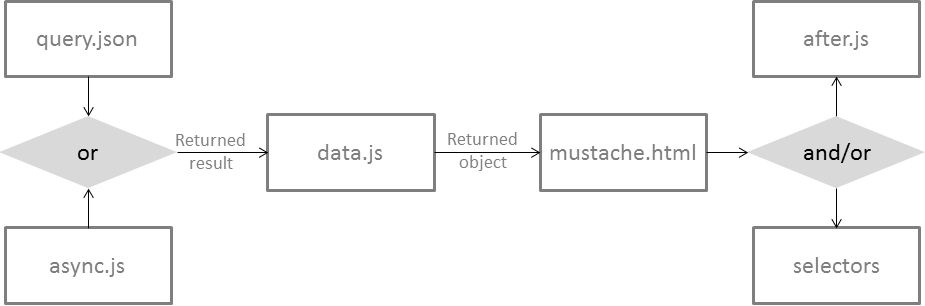
\includegraphics[width=1.00\columnwidth]{images/eventlyeventhandler.png}
\caption{Illustration of Evently's event handling}
\label{img:eventlyeventhandler}
\end{figure}
Actually, all the event handler's components need not to be defined in a certain folder structure, but can be defined in a single JSON file (i.e. all components are attributes of an event handler object). However, for the sake of clarity, the described approach is recommended.\\
Firing an event is done via a function provided by Evently. In the following example the \emph{this} keyword refers to the current widget (the "menu" from above), for which the event "menuitemselected" is triggered:
\begin{lstlisting}
$.couch.app(function (app) {
  $(this).trigger("menuitemselected");
});
\end{lstlisting}

\section{LabLOUNGE from a user's perspective}
\label{couchapp:labloungeuser}
To demonstrate the communication of a client with LabVIEW via CouchDB, we implemented a prototypical CouchApp named \emph{LabLOUNGE}\footnote{\url{https://github.com/treschenhofer/lablounge}}.\\
The LabLOUNGE page consist of three widgets:
\begin{description}
\item[main] The main content on the left side of the page, which shows either a device's data as time series (see Figure~\ref{img:lablounge01}), or a form for the submission of notifications to LabVIEW (see Figure~\ref{img:lablounge02}).
\begin{figure}[h!]
\centering
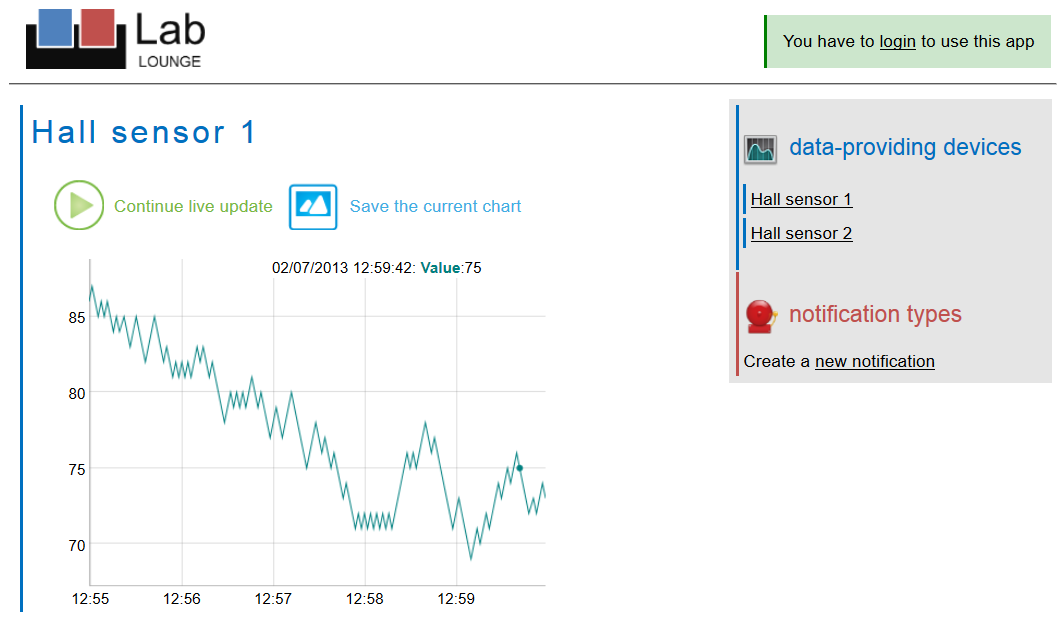
\includegraphics[width=1.0\columnwidth]{images/lablounge01.png}
\caption{The LabLOUNGE CouchApp in "plotting mode", showing a device's data as time series}
\label{img:lablounge01}
\end{figure}

\begin{figure}[h!]
\centering
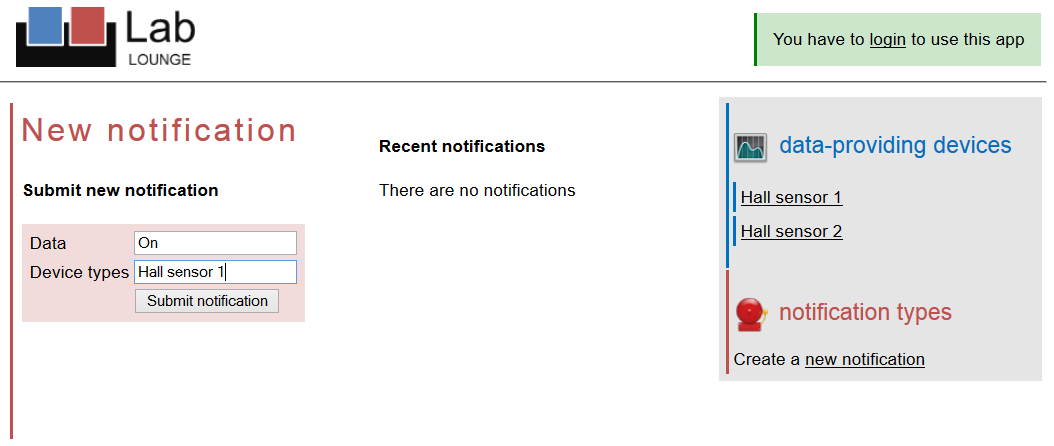
\includegraphics[width=1.0\columnwidth]{images/lablounge02.png}
\caption{The LabLOUNGE CouchApp in "notification mode", showing a form for the submission of notifications}
\label{img:lablounge02}
\end{figure}

\item[data-providing devices] A list of devices on the upper right side of the page, which contains all devices, for which there is at least one data entry in the database.

\item[notification types] A list of already submitted notifications grouped by their type on the lower right side of the page. Moreover, this widget contains a link to create a new notification.
\end{description}

\subsection{Time series}
As shown in Figure~\ref{img:lablounge01}, a device's data is represented as time series in a chart. This chart supports a live update feature, i.e. if a measuring device creates a permanent data stream, the changes feed of CouchDB can be used to respond to these changes by automatically updating the chart.\\
However, to save the chart as an image, the user can pause the live update to freeze the chart in order to open the chart as an image, which can be saved via the browser's "Save image as..." menu (see Figure~\ref{img:labloungechart}).\\
\begin{figure}[h!]
\centering
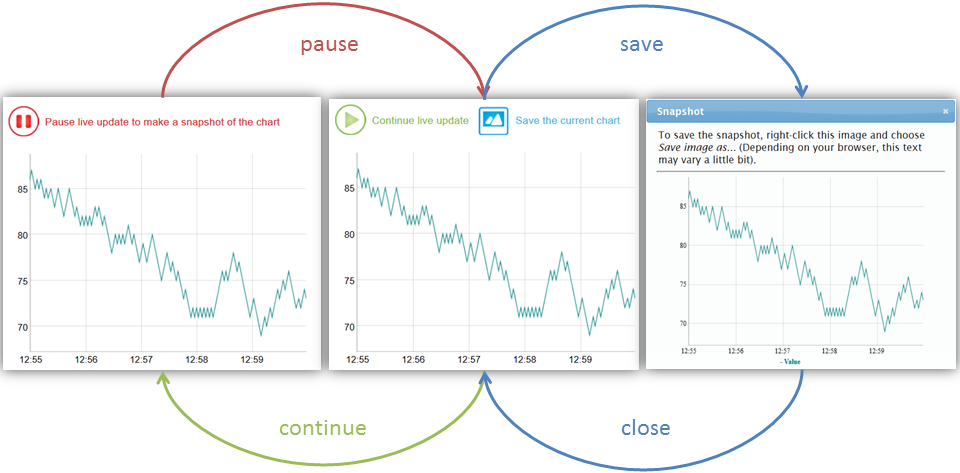
\includegraphics[width=1.0\columnwidth]{images/labloungechart.png}
\caption{A device's data plotted as a time series, which can be saved as an image}
\label{img:labloungechart}
\end{figure}
The live update can be reactivated at any time, s.t. each data set, which was created while the chart was frozen, is reloaded to update the chart.

\subsection{Notifications}
To send a notification via the CouchDB to LabLOUNGE, the user can either select an already existing notification type to resend a previously sent notification (see Figure~\ref{img:labloungenotification}), or create a new one.\\
\begin{figure}[h!]
\centering
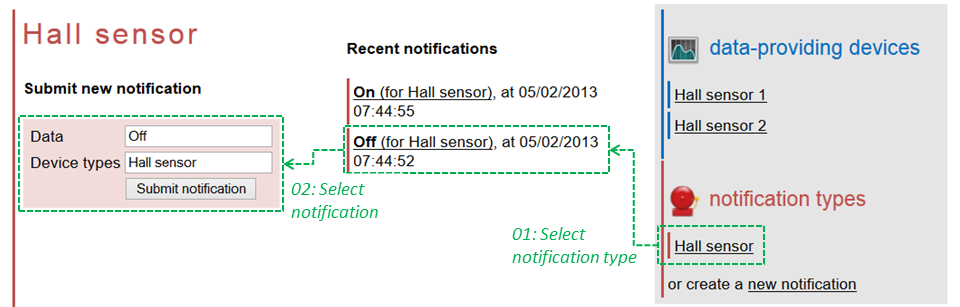
\includegraphics[width=1.0\columnwidth]{images/labloungenotification.png}
\caption{Creation of a new notification based on previously sent ones}
\label{img:labloungenotification}
\end{figure}

\section{LabLOUNGE from a developer's perspective}
\label{couchapp:labloungedeveloper}
The source project of our prototypical implementation can be found at GitHub\footnote{\url{https://github.com/treschenhofer/lablounge}} and opened with Visual Studio 2012. A CouchApp's structure and hence LabLOUNGE's project structure was already explained in Section~\ref{couchapp:development}.\\
As mentioned in the previous section, LabLOUNGE consists of three widgets: \emph{main}, \emph{devices}, and \emph{notificationtypes}. Their position on the page is defined in "index.html", which contains the associations of div elements with corresponding Evently widgets on the one hand, and the definition of widget connections on the other hand:
\begin{lstlisting}
$.couch.app(function (app) {
  $("#main").evently("main", app);
  $("#registereddevices").evently("devices", app);
  $("#notificationtypes").evently("notificationtypes", app);

  $.evently.connect("#registereddevices", "#main", 
		["deviceselected"]);
  $.evently.connect("#notificationtypes", "#main", 
		["notificationtypeselected"]);
});
\end{lstlisting}

\subsection{\emph{devices} widget}
\label{couchapp:labloungedeveloper:devices}
\begin{figure}[h!]
\centering
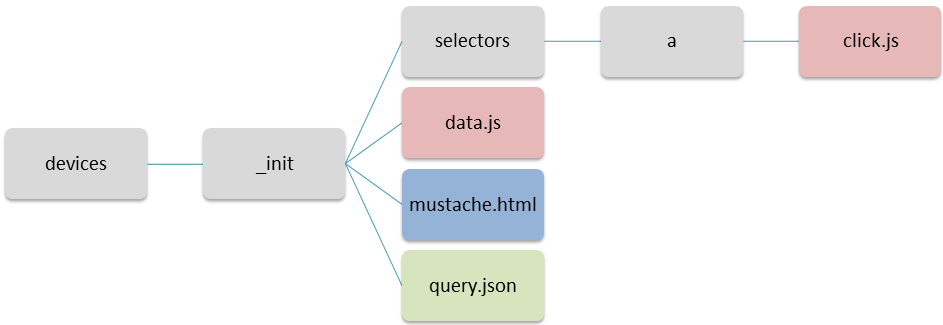
\includegraphics[width=1.0\columnwidth]{images/labloungestructuredevices.png}
\caption{Folder structure of the \emph{devices} widget}
\label{img:structuredevices}
\end{figure}
As shown in Figure~\ref{img:structuredevices}, this widget consists just of the "\_init" event handler. Therefore, when loading LabLOUNGE, this widget performs the query defined in "query.json", which is the predefined query "dataprovidingdevices" determining all devices providing at least one data entry.\\
The results are processed in data.js and forwarded to the mustache template, which generates a hyperlink (anchor) for each of the obtained devices. The selector defined in the widget applies to all of these anchors and handles their click events by storing the selected device onto the page and triggering the custom event "deviceselected", which will be handled by the \emph{main} widget (see Subsection~\ref{couchapp:labloungedeveloper:main}).

\subsection{\emph{notificationtypes} widget}
\label{couchapp:labloungedeveloper:notificationtypes}
\begin{figure}[h!]
\centering
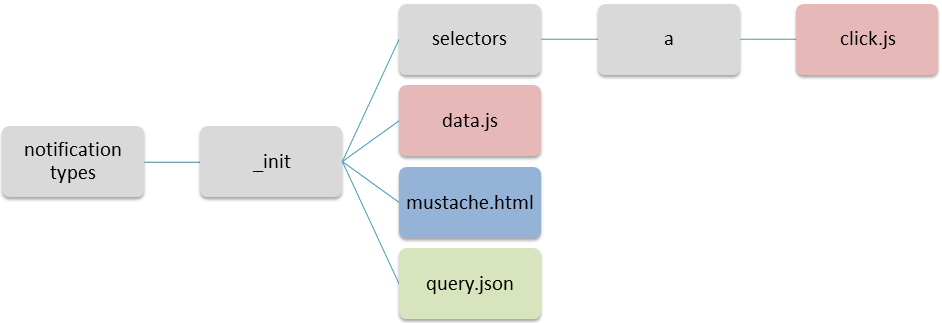
\includegraphics[width=1.0\columnwidth]{images/labloungestructurenotificationtypes.png}
\caption{Folder structure of the \emph{notificationtypes} widget}
\label{img:structurenotificationtypes}
\end{figure}
This widget's structure (depicted in Figure~\ref{img:structurenotificationtypes}) is very similar to the structure of the \emph{devices} widget. Again, there is just an "\_init" event handler, performing the predefined query "notificationtypes" when loading LabLOUNGE. This query determines all notification types, for which there is at least one notification instance.\\
Via the data function, these notification types are passed to the mustache template, which shows them as a list of anchors. Moreover, the template also defines a hyperlink for the creation of a new notification. Similar to the \emph{devices} widget, the selector in the \emph{notificationtypes} widget applies to all its anchors and handles the click events of them by storing the selected notification type onto the page and triggering the custom event "notificationtypeselected".
\subsection{\emph{main} widget}
\label{couchapp:labloungedeveloper:main}
\begin{figure}[h!]
\centering
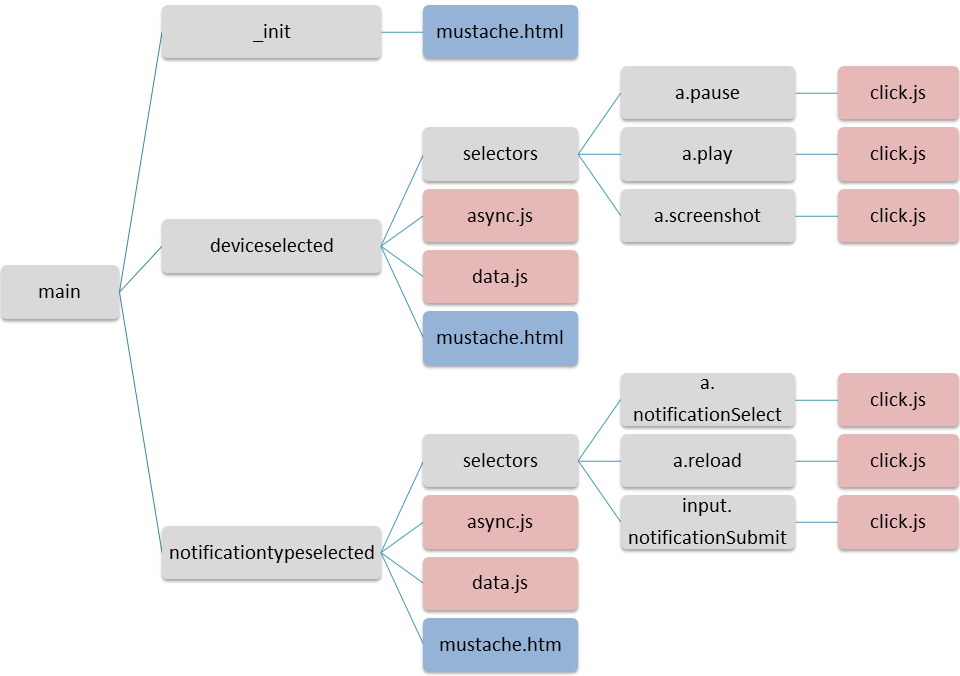
\includegraphics[width=1.0\columnwidth]{images/labloungestructuremain.png}
\caption{Folder structure of the \emph{main} widget}
\label{img:structuremain}
\end{figure}
As illustrated in Figure~\ref{img:structuremain}, the \emph{main} widget is the most complex one, since it consists of the three event handlers "\_init", "deviceselected", and "notifiationtypeselected".\\
The initial state of the \emph{main} widget is defined by the "\_init" event handler. However, since there is nothing to display before the selection of either a device or a notification type, this event handler consists only of a mustache template defining a simple static text.

\subsubsection{"deviceselected" event handler}
\label{couchapp:labloungedeveloper:main:deviceselected}
If the user selects a device in the \emph{devices} widget, the event "deviceselected" is triggered, which is handled by this event handler.\\
First, the async function determines the selected device and performs a query obtaining all the device's entries in reversed chronological order (the reversed order simplifies the adding of new entries by the live update feature). Furthermore, this function activates live update, i.e. LabLOUNGE will listen to the changes feed to immediately gather new created data entries.\\
After some processing of the obtained data in the data function, it is passed to the mustache template, where it is plotted as a time series, whereas plotting is done by the JavaScript Visualization library \emph{dygraphs}\footnote{\url{http://dygraphs.com}}. Moreover, the JavaScript library \emph{Moment.js}\footnote{\url{http://momentjs.com}} is used for the processing of datetime values.\\
The "deviceselected" event handler consists of three selectors:
\begin{description}
\item[a.pause] Handles the click event for the pause button. Stops the live update and showing buttons to continue the live update as well as to save the frozen chart.
\item[a.play] Handles the click event for the pause button. Continues the live update
\item[a.screenshot] Handles the click event for the save button. Opens a jQuery UI modal pop-up providing the frozen chart as a downloadable image.
\end{description}
The most interesting part of this widget is the live update feature, which is implemented in "\_attachments/logic.js".\\
On each change of the database's data this function is called, which is defined by the following lines of code:
\begin{lstlisting}
$dbname = "lablounge";
$appname = "labLounge";
$db = $.couch.db($dbname);
$db.changes().onChange(onDBChange);

function onDBChange(data) {
  ...
}
\end{lstlisting}
Since this function is invoked on EACH change of the database, it has to evaluate the relevance of the change for the live update feature by checking the following conditions:
\begin{itemize}
	\item Is currently any device selected at all, i.e. is LabLOUNGE in "plotting mode" (as in Figure~\ref{img:lablounge01}) or in "notification mode" (as in Figure~\ref{img:lablounge02})?
	\item Is live update activated or deactivated?
	\item Is the changed database document a data entry?
	\item And if yes, belongs this data entry to the selected device?
\end{itemize}

If the answer to all of these questions is "Yes", the new data entry is added to the plot.

\subsubsection{"notifiationtypeselected" event handler}
\label{couchapp:labloungedeveloper:main:notifiationtypeselected}
If the user selects a notification type in the \emph{notification type} widget, the event "notificationtypeselected" is triggered, which is handled by this event handler.\\
Similar to the "deviceselected" event handler, the async function first determines the selected notification type and performs a query obtaining all existing notification instances for the given type in reversed chronological order.\\
After some processing in the data function of this event handler, the obtained notifications are passed to the mustache template, which displays them as a list of anchors on the right side of the \emph{main} widget, and showing a form to submit a new notification on the left side of the \emph{widget} (see Figure~\ref{img:labloungenotification}).\\
The "a.notificationSelect" selector handles the click event of the anchors in the "Recent notifications" link by filling the form on the left side with the data of the chosen notification. The submission of a new notification is handled by the "input.notificationSubmit" selector, which creates a new notification object by the form data and saves this object as a document in the CouchDB:
\begin{lstlisting}
var notification =
{
  types : $("#deviceTypesDataField").val().split(","),
  data: $("#notificationDataField").val(),
  ...
};

$db.saveDoc(notification,
{
  success:function(data) {
    ...
  },
  error:function(ex){
    ...
  }
});
\end{lstlisting}
		%\chapter{Conclusion}

		
	%\bibliographystyle{styles/plain.bst}
  \bibliography{bibliography/literature}
		% ---------------------------------------------------------------------------
		%
		% Appendix
		%
		% ---------------------------------------------------------------------------
		
		%\part*{Appendix}
		\newpage
		%\addcontentsline{toc}{part}{Appendix}
		
		
		
		%\appendix %---------------------------------------
\chapter{Appendix}
\section{Attached files}

		
	  \clearemptydoublepage
	
 
\end{document}

